\documentclass[colorlinks,11pt,a4paper,normalphoto,withhyper,ragged2e]{altareport}


%%%%%%%%%%%%%%%%%%%%%%%%%%%%%%%%%%%%%%%%%%%
%%%%%%%%%% DEFAULT PACKAGES & SETTINGS %%%%%%%%%%
\usepackage[utf8]{inputenc}
\usepackage{setspace} %1.5 line spacing
\usepackage{notoccite} %% Citation numbering
\usepackage{lscape} %% Landscape table
\usepackage{caption} %% Adds a newline in the table caption

%% The paracol package lets you typeset columns of text in parallel
\usepackage{paracol}
\usepackage[none]{hyphenat}

%% Document and Theme Fonts
\usepackage[T1]{fontenc}
\usepackage{paratype}
\usepackage[defaultsans]{lato}
%\usepackage[sfdefault,light,condensed]{roboto}
%\usepackage[rm]{roboto}
%\usepackage[defaultsans]{lato}
%\usepackage{sourcesanspro}
%\usepackage[rm]{merriweather}

\setlength{\intextsep}{4pt} % Set defualt spacing around floats

%%%%%%%%%%%%%%%%%%%%%%%%%%%%%%%%%%%%%%%%%%%


%%%%%%%%%%%%%%%%%%%%%%%%%%%%%%%%%%%%%%%%%%%
%%%%%%%%%% THEMES %%%%%%%%%%

%% Standard theme options are below, leave blank for B&W / no colours (BoringDefault). Note the theme will be set to default if you enter a non-exsistant theme name.
\SetTheme{UNILIM}
%% UNILIM
%% PastelBlue
%% GreenAndGold
%% Purple
%% PastelRed
%% BoringDefault (Leave blank / enter anything not found above)

%%%%%%%%%%%%%%%%%%%%%%%%%%%%%%%%%%%%%%%%%%%






%%%%%%%%%%%%%%%%%%%%%%%%%%%%%%%%%%%%%%%%%%%
%%%%%%%%%% DOCUMENT SPECIFIC PACKAGES %%%%%%%%%%

\usepackage{amssymb}
\usepackage{amsfonts}
\usepackage{mathtools}

\usepackage{pythontex} % Run python code in this latex doc

%%%%%%%%% Karnaugh Map Package & Settings %%%%%%%%%
\usepackage[export]{adjustbox}

\usetikzlibrary{matrix,calc}
\usepackage{karnaugh-map}

\colorlet{LightRed}{red!60!}
\colorlet{LightBlue}{blue!60!}
\colorlet{LightYellow}{yellow!60!}
\colorlet{LightGreen}{green!60!}
\colorlet{LightOrange}{orange!60!}

%%%%%%%%% MATLAB Language Settings %%%%%%%%%
\usepackage[numbered,framed]{matlab-prettifier} % To add code listings from matlab
\lstMakeShortInline[style=Matlab-editor]" %% This makes " an escape character to write in matlab editor font

%%%%%%%%% Arduino Language Settings %%%%%%%%%
\lstset{%
  language = Octave,
  backgroundcolor=\color{white},   
  basicstyle=\color{body}\footnotesize\ttfamily,       
  %breakatwhitespace=false,         
  breaklines=true,                                
  commentstyle=\color{CommentGreen},
  columns=fullflexible,
  escapeinside={\%*}{*)},
  extendedchars=true,
  frame=leftline,
  keepspaces=true,
  keywordstyle=\color{LightBlue},
  numbersep=5pt,
  numberstyle=\footnotesize\color{gray},
  rulecolor=\color{black},
  rulesepcolor=\color{black},
  showtabs=true,
  stringstyle=\color{LightBlue},
  tabsize=2,                       
  title=\lstname,
  emphstyle=\bfseries\color{LightOrange}%  style for emph={} 
} 

%%%%% language/example specific settings: %%%%%
\lstdefinestyle{Arduino}{%
    language = C++,
    keywords={void, int, boolean, char, unsigned, long, uint32_t, volatile, byte, uint8_t, HIGH, OUTPUT, LOW, INPUT},%                 define keywords
    morecomment=[l]{//},%             treat // as comments
    morecomment=[s]{/*}{*/},%         define /* ... */ comments
    emph={WiFi, Serial, IPAddress, Adafruit_NeoPixel, setFrequency, println, print, delay, digitalWrite, pinMode, available, digitalPinToInterrupt, attachInterrupt, detachInterrupt, analogRead, NEO_GRB, NEO_KHZ800, noInterrupts, interrupts, strstr, endPacket, beginPacket, remoteIP, remotePort, APClientMacAddress, Color}%        keywords to emphasize
}


%%%%% Settings for python pgf graphs %%%%%
\usepackage{pgfplots}
\usetikzlibrary{arrows.meta}

\pgfplotsset{compat=newest,
    width=6cm,
    height=3cm,
    scale only axis=true,
    max space between ticks=25pt,
    try min ticks=5,
    every axis/.style={
        axis y line=left,
        axis x line=bottom,
        axis line style={thick,->,>=latex, shorten >=-.4cm}
    },
    every axis plot/.append style={thick},
    tick style={black, thick}
}
\tikzset{
    semithick/.style={line width=0.8pt},
}

\usepgfplotslibrary{groupplots}
\usepgfplotslibrary{dateplot}


% Reduce space around captions
% \captionsetup{aboveskip=5pt, belowskip=5pt}
%%%%%%%%%%%%%%%%%%%%%%%%%%%%%%%%%%%%%%%%%%%




%%%%%%%%%%%%%%%%%%%%%%%%%%%%%%%%%%%%%%%%%%%
%%%%%%%%%% USEFUL SETTINGS %%%%%%%%%%
%% Change some font sizes, this will override the defaults
\renewcommand{\ReportTitleFont}{\Huge\rmfamily\bfseries} %% Title Page - Main Title
\renewcommand{\ReportSubTitleFont}{\huge\bfseries} %% Title Page - Sub-Title
\renewcommand{\ReportSectionFont}{\LARGE\rmfamily\bfseries} %% Section Title
\renewcommand{\ReportSubSectionFont}{\large\bfseries} %% SubSection Title
\renewcommand{\FootNoteFont}{\footnotesize} %% Footnotes and Header/Footer

%% Change the bullets for itemize and rating marker
\renewcommand{\itemmarker}{{\small\textbullet}}
\renewcommand{\ratingmarker}{\faCircle}

%% Change the page layout
\geometry{left=1.5cm,right=1.5cm,top=3cm,bottom=3cm,columnsep=8mm}
\onehalfspace   % 1.5 line spacing

\definecolor{CommentGreen}{HTML}{228B22}
%%%%%%%%%%%%%%%%%%%%%%%%%%%%%%%%%%%%%%%%%%%




%%%%%%%%%%%%%%%%%%%%%%%%%%%%%%%%%%%%%%%%%%%
\include{references.bib}

%%%%%%%%%% TITLE PAGE INFO %%%%%%%%%%
\ReportTitle{Fundamentals of Coherent Photonics}
\SubTitle{Linear Propagation in Optical Wave-guides - Notes \& Tutorials}
\Author{Andrew Simon Wilson}
\ReportDate{\today}
\FacultyOrLocation{EMIMEO Programme}
\ModCoord{Dr. Diominique Pagnoux}

%%%%%%%%%%%%%%%%%%%%%%%%%%%%%%%%%%%%%%%%%%%


\newcommand*\circled[1]{\tikz[baseline=(char.base)]{
            \node[shape=circle,draw,inner sep=0.5pt] (char) {#1};}}


\begin{document}

\MakeReportTitlePage


%%%%% CONTENTS %%%%%
\pagenumbering{roman} % Start roman numbering
\setcounter{page}{1}


%%%%%%%%%% YOUR NAME, PROFESSION, PORTRAIT, CONTACT INFO, SOCIAL MEDIA ETC. %%%%%%%%%%
\name{Andrew Simon Wilson, BEng}
\tagline{Post-graduate Master's Student, Erasmus Mundus JMD - EMIMEO Programme}

\personalinfo{
  \email{andrew.wilson@etu.unilim.fr}
  \linkedin{andrew-simon-wilson} 
  \github{AS-Wilson}
  \phone{+44 7930 560 383}
}

%% You can add multiple photos on the left or right
% \photoR{3cm}{Images/a-wilson-potrait.jpg}
% \photoL{3cm}{Yacht_High,Suitcase_High}


\section*{Author Details}
\makeauthordetails

%% Table of contents print level -1: part, 0: chapter, 1: section, 2:sub-section, 3:sub-sub-section, etc.
\setcounter{tocdepth}{2} 
\tableofcontents %% Prints a list of all sections based on the above command
%\listoffigures %% Prints a list of all figures in the report
%\listoftables %% Prints a list of all tables in the report




%%%%%%%%%% DOCUMENT CONTENT BEGINS HERE %%%%%%%%%%

%%%%% INTRO %%%%%
\section*{Introduction}
What is the rational behind this document, why would I make it? \linebreak
Put simply, I like to have a permanent and archive-able copy of my work and for it to be in a presentable format. This results in easy revision, ensures I have fully explored the topic and questions, and provides an easy to read way for professors to check my understanding and to give others help with the topic. \linebreak 
I spent have spent a lot of time developing the template used to make this {\LaTeX} document, I want others to benefit from this work so the source code for this template is available on GitHub \cite{JenningsWilson2021}.
\newpage
\pagenumbering{arabic} % Start document numbering - roman numbering




\section{Class Notes, Study Notes, and Revision}







\paragraph{Modes \linebreak}
The modes of light in a fibre correspond to the solutions that can be found to Maxwell's field equations for the distribution of the electric and magnetic fields within the fibre. \linebreak

Once we obtain a differential equation which describes the EM field's components it's surface is able to be solved by using the bessel functions (which are particularly applicable to the components of cylindrically shaped phenomena in engineering in general). Unless weakly guided, each mode will be described by a given bessel function??





\paragraph{LP Mode Electric Field Distributions \linebreak}





\paragraph{The propagation constant, $\boldsymbol{\beta}$ \linebreak}
Firstly, please note this is sometimes (extremely confusingly) referred to as the wavenumber in some textbooks (and vice-versa, the wavenumber is called the propagation constant). However, in the case of these notes this will always be the propagation constant (with the wavenumber being something else entirely, described in these notes elsewhere, and denoted $k$). measured in $m^{-1}$

Denoted $\beta$ 

each mode will result in a different solution to it's propagation constant (sometimes called a wavenumber in textbooks), 

\columnratio{0.2}
%%%%%%%%%% LEFT HAND COLUMN %%%%%%%%%%
% Start a 2-column paracol. Both the left and right columns will automatically
% break across pages if things get too long.
\begin{paracol}{2}

\medskip

\setlength{\jot}{2ex}
\begin{align}
	\beta &= \nonumber
\end{align}

%%%%%%%%%% RIGHT HAND COLUMN %%%%%%%%%%
%% Switch to the right column. This will now automatically move to the second
%% page if the content is too long.
\switchcolumn

\setlength{\jot}{1ex}
\begin{align}
	\text{Where:}& \nonumber\\
	\beta & \text{ is something} \nonumber
\end{align}

\end{paracol}




\paragraph{The wavenumber, $\textbf{k}$ \linebreak}



\columnratio{0.2}
%%%%%%%%%% LEFT HAND COLUMN %%%%%%%%%%
% Start a 2-column paracol. Both the left and right columns will automatically
% break across pages if things get too long.
\begin{paracol}{2}

\medskip

\setlength{\jot}{2ex}
\begin{align}
	k &= \frac{\omega}{c} = \frac{2\pi\nu}{c} \nonumber\\
	&= \frac{2\pi}{\lambda} = nk_0 \nonumber
\end{align}

%%%%%%%%%% RIGHT HAND COLUMN %%%%%%%%%%
%% Switch to the right column. This will now automatically move to the second
%% page if the content is too long.
\switchcolumn

\setlength{\jot}{1ex}
\begin{align}
	\text{Where:}& \nonumber\\
	\omega & \text{ (greek letter ``omega'') is the angular, optical frequency in Radians/Second} \nonumber\\
	\nu & \text{ (greek letter ``nu'') is the periodic frequency in Hertz} \nonumber\\
	c & \text{ is the speed } \nonumber\\
	\lambda & \text{ (greek letter ``lambda'') is the wavelength of the light in metres} \nonumber	
\end{align}

\end{paracol}




\paragraph{The ``V'' Parameter, ``Fibre'' Parameter or Normalised Spatial Frequency, $\textbf{V}$ \linebreak}

 and governs the number of modes able 

\columnratio{0.2}
%%%%%%%%%% LEFT HAND COLUMN %%%%%%%%%%
% Start a 2-column paracol. Both the left and right columns will automatically
% break across pages if things get too long.
\begin{paracol}{2}

\medskip

\setlength{\jot}{2ex}
\begin{align}
	V = \frac{2 \pi a}{\lambda}\sqrt{n_{core}^2 - n_{clad}^2} \nonumber
\end{align}

%%%%%%%%%% RIGHT HAND COLUMN %%%%%%%%%%
%% Switch to the right column. This will now automatically move to the second
%% page if the content is too long.
\switchcolumn

\setlength{\jot}{1ex}
\begin{align}
	\text{Where:}& \nonumber\\\
	\lambda & \text{ is the wavelength of the light propagating down the fibre} \nonumber\\\
	n_{core} & \text{ is the refractive index of the core's material (unitless)} \nonumber\\\
	n_{clad} & \text{ is the refractive index of the cladding's material (unitless)} \nonumber\\\
	V & \text{ is the normalised spatial frequency, the fibre parameter, or the ``V'' parameter} \nonumber\
\end{align}

\end{paracol}



\begin{align}
	\text{Where:}& \nonumber\\\
	\bar{\Theta}_c & \text{ is the critical angle for rays to make total internal reflections at the core-cladding boundary (Radians)} \nonumber\
\end{align}




\newpage




\section{Tutorials}
%%%%% TUTORIAL ONE %%%%%
\subsection{Tutorial One - Propagation of LP Modes in Step Index Fibres}
%%%%% QUESTION ONE %%%%%
\subsubsection{Question One}
\textit{Step index fibres are constituted by a cylindrical core refractive index n\textsubscript{1}($\lambda$), surrounded by a cladding refractive index n\textsubscript{2}($\lambda$). Most of the time, the cladding is masde of pure silica and the core is made of silica doped with germanium.} \\


\paragraph{Part A \linebreak}
\textit{What is the meaning of the expression ``Step Index''?} \linebreak


%% Set the left/right column width ratio to 6:4.
\columnratio{0.6}

%%%%%%%%%% LEFT HAND COLUMN %%%%%%%%%%
% Start a 2-column paracol. Both the left and right columns will automatically
% break across pages if things get too long.
\begin{paracol}{2}

``Step Index'' refers to the refractive index profile of the core and the difference between the core and cladding refractive indices (usually denoted $n_1$ and $n_2$ respectively). In a step index fibre the index of the core remains constant through it's radius and then the refractive index value ``steps'' immediately at the cladding.

Figure \ref{fig:fibre_index_profile} shows the cross section of a step index fibre (on the left of the image) and a graph plotting refractive index versus cross-sectional radius, the x-axis represents the refractive index as it varies against the radius of the cross section (represented by the y-axis).


%%%%%%%%%% RIGHT HAND COLUMN %%%%%%%%%%
%% Switch to the right column. This will now automatically move to the second
%% page if the content is too long.
\switchcolumn

\begin{figure}[h]
	\centering
	\scalebox{0.4}{%% Creator: Matplotlib, PGF backend
%%
%% To include the figure in your LaTeX document, write
%%   \input{<filename>.pgf}
%%
%% Make sure the required packages are loaded in your preamble
%%   \usepackage{pgf}
%%
%% Figures using additional raster images can only be included by \input if
%% they are in the same directory as the main LaTeX file. For loading figures
%% from other directories you can use the `import` package
%%   \usepackage{import}
%%
%% and then include the figures with
%%   \import{<path to file>}{<filename>.pgf}
%%
%% Matplotlib used the following preamble
%%   \usepackage[T1]{fontenc} \usepackage{mathpazo}
%%
\begingroup%
\makeatletter%
\begin{pgfpicture}%
\pgfpathrectangle{\pgfpointorigin}{\pgfqpoint{6.412831in}{3.424221in}}%
\pgfusepath{use as bounding box, clip}%
\begin{pgfscope}%
\pgfsetbuttcap%
\pgfsetmiterjoin%
\definecolor{currentfill}{rgb}{1.000000,1.000000,1.000000}%
\pgfsetfillcolor{currentfill}%
\pgfsetlinewidth{0.000000pt}%
\definecolor{currentstroke}{rgb}{1.000000,1.000000,1.000000}%
\pgfsetstrokecolor{currentstroke}%
\pgfsetdash{}{0pt}%
\pgfpathmoveto{\pgfqpoint{0.000000in}{0.000000in}}%
\pgfpathlineto{\pgfqpoint{6.412831in}{0.000000in}}%
\pgfpathlineto{\pgfqpoint{6.412831in}{3.424221in}}%
\pgfpathlineto{\pgfqpoint{0.000000in}{3.424221in}}%
\pgfpathclose%
\pgfusepath{fill}%
\end{pgfscope}%
\begin{pgfscope}%
\pgfsetbuttcap%
\pgfsetmiterjoin%
\definecolor{currentfill}{rgb}{0.933333,0.933333,0.933333}%
\pgfsetfillcolor{currentfill}%
\pgfsetlinewidth{0.000000pt}%
\definecolor{currentstroke}{rgb}{0.000000,0.000000,0.000000}%
\pgfsetstrokecolor{currentstroke}%
\pgfsetstrokeopacity{0.000000}%
\pgfsetdash{}{0pt}%
\pgfpathmoveto{\pgfqpoint{0.617463in}{0.490733in}}%
\pgfpathlineto{\pgfqpoint{3.308449in}{0.490733in}}%
\pgfpathlineto{\pgfqpoint{3.308449in}{3.181720in}}%
\pgfpathlineto{\pgfqpoint{0.617463in}{3.181720in}}%
\pgfpathclose%
\pgfusepath{fill}%
\end{pgfscope}%
\begin{pgfscope}%
\pgfpathrectangle{\pgfqpoint{0.617463in}{0.490733in}}{\pgfqpoint{2.690987in}{2.690987in}}%
\pgfusepath{clip}%
\pgfsetbuttcap%
\pgfsetroundjoin%
\pgfsetlinewidth{0.501875pt}%
\definecolor{currentstroke}{rgb}{0.698039,0.698039,0.698039}%
\pgfsetstrokecolor{currentstroke}%
\pgfsetdash{{1.850000pt}{0.800000pt}}{0.000000pt}%
\pgfpathmoveto{\pgfqpoint{0.927961in}{0.490733in}}%
\pgfpathlineto{\pgfqpoint{0.927961in}{3.181720in}}%
\pgfusepath{stroke}%
\end{pgfscope}%
\begin{pgfscope}%
\pgfsetbuttcap%
\pgfsetroundjoin%
\definecolor{currentfill}{rgb}{0.180392,0.180392,0.180392}%
\pgfsetfillcolor{currentfill}%
\pgfsetlinewidth{0.803000pt}%
\definecolor{currentstroke}{rgb}{0.180392,0.180392,0.180392}%
\pgfsetstrokecolor{currentstroke}%
\pgfsetdash{}{0pt}%
\pgfsys@defobject{currentmarker}{\pgfqpoint{0.000000in}{-0.048611in}}{\pgfqpoint{0.000000in}{0.000000in}}{%
\pgfpathmoveto{\pgfqpoint{0.000000in}{0.000000in}}%
\pgfpathlineto{\pgfqpoint{0.000000in}{-0.048611in}}%
\pgfusepath{stroke,fill}%
}%
\begin{pgfscope}%
\pgfsys@transformshift{0.927961in}{0.490733in}%
\pgfsys@useobject{currentmarker}{}%
\end{pgfscope}%
\end{pgfscope}%
\begin{pgfscope}%
\definecolor{textcolor}{rgb}{0.180392,0.180392,0.180392}%
\pgfsetstrokecolor{textcolor}%
\pgfsetfillcolor{textcolor}%
\pgftext[x=0.927961in,y=0.393510in,,top]{\color{textcolor}\rmfamily\fontsize{11.000000}{13.200000}\selectfont \(\displaystyle {\ensuremath{-}50}\)}%
\end{pgfscope}%
\begin{pgfscope}%
\pgfpathrectangle{\pgfqpoint{0.617463in}{0.490733in}}{\pgfqpoint{2.690987in}{2.690987in}}%
\pgfusepath{clip}%
\pgfsetbuttcap%
\pgfsetroundjoin%
\pgfsetlinewidth{0.501875pt}%
\definecolor{currentstroke}{rgb}{0.698039,0.698039,0.698039}%
\pgfsetstrokecolor{currentstroke}%
\pgfsetdash{{1.850000pt}{0.800000pt}}{0.000000pt}%
\pgfpathmoveto{\pgfqpoint{1.962956in}{0.490733in}}%
\pgfpathlineto{\pgfqpoint{1.962956in}{3.181720in}}%
\pgfusepath{stroke}%
\end{pgfscope}%
\begin{pgfscope}%
\pgfsetbuttcap%
\pgfsetroundjoin%
\definecolor{currentfill}{rgb}{0.180392,0.180392,0.180392}%
\pgfsetfillcolor{currentfill}%
\pgfsetlinewidth{0.803000pt}%
\definecolor{currentstroke}{rgb}{0.180392,0.180392,0.180392}%
\pgfsetstrokecolor{currentstroke}%
\pgfsetdash{}{0pt}%
\pgfsys@defobject{currentmarker}{\pgfqpoint{0.000000in}{-0.048611in}}{\pgfqpoint{0.000000in}{0.000000in}}{%
\pgfpathmoveto{\pgfqpoint{0.000000in}{0.000000in}}%
\pgfpathlineto{\pgfqpoint{0.000000in}{-0.048611in}}%
\pgfusepath{stroke,fill}%
}%
\begin{pgfscope}%
\pgfsys@transformshift{1.962956in}{0.490733in}%
\pgfsys@useobject{currentmarker}{}%
\end{pgfscope}%
\end{pgfscope}%
\begin{pgfscope}%
\definecolor{textcolor}{rgb}{0.180392,0.180392,0.180392}%
\pgfsetstrokecolor{textcolor}%
\pgfsetfillcolor{textcolor}%
\pgftext[x=1.962956in,y=0.393510in,,top]{\color{textcolor}\rmfamily\fontsize{11.000000}{13.200000}\selectfont \(\displaystyle {0}\)}%
\end{pgfscope}%
\begin{pgfscope}%
\pgfpathrectangle{\pgfqpoint{0.617463in}{0.490733in}}{\pgfqpoint{2.690987in}{2.690987in}}%
\pgfusepath{clip}%
\pgfsetbuttcap%
\pgfsetroundjoin%
\pgfsetlinewidth{0.501875pt}%
\definecolor{currentstroke}{rgb}{0.698039,0.698039,0.698039}%
\pgfsetstrokecolor{currentstroke}%
\pgfsetdash{{1.850000pt}{0.800000pt}}{0.000000pt}%
\pgfpathmoveto{\pgfqpoint{2.997951in}{0.490733in}}%
\pgfpathlineto{\pgfqpoint{2.997951in}{3.181720in}}%
\pgfusepath{stroke}%
\end{pgfscope}%
\begin{pgfscope}%
\pgfsetbuttcap%
\pgfsetroundjoin%
\definecolor{currentfill}{rgb}{0.180392,0.180392,0.180392}%
\pgfsetfillcolor{currentfill}%
\pgfsetlinewidth{0.803000pt}%
\definecolor{currentstroke}{rgb}{0.180392,0.180392,0.180392}%
\pgfsetstrokecolor{currentstroke}%
\pgfsetdash{}{0pt}%
\pgfsys@defobject{currentmarker}{\pgfqpoint{0.000000in}{-0.048611in}}{\pgfqpoint{0.000000in}{0.000000in}}{%
\pgfpathmoveto{\pgfqpoint{0.000000in}{0.000000in}}%
\pgfpathlineto{\pgfqpoint{0.000000in}{-0.048611in}}%
\pgfusepath{stroke,fill}%
}%
\begin{pgfscope}%
\pgfsys@transformshift{2.997951in}{0.490733in}%
\pgfsys@useobject{currentmarker}{}%
\end{pgfscope}%
\end{pgfscope}%
\begin{pgfscope}%
\definecolor{textcolor}{rgb}{0.180392,0.180392,0.180392}%
\pgfsetstrokecolor{textcolor}%
\pgfsetfillcolor{textcolor}%
\pgftext[x=2.997951in,y=0.393510in,,top]{\color{textcolor}\rmfamily\fontsize{11.000000}{13.200000}\selectfont \(\displaystyle {50}\)}%
\end{pgfscope}%
\begin{pgfscope}%
\definecolor{textcolor}{rgb}{0.180392,0.180392,0.180392}%
\pgfsetstrokecolor{textcolor}%
\pgfsetfillcolor{textcolor}%
\pgftext[x=1.962956in,y=0.184339in,,top]{\color{textcolor}\rmfamily\fontsize{13.200000}{15.840000}\selectfont y Dimension (\(\displaystyle \mu\)m)}%
\end{pgfscope}%
\begin{pgfscope}%
\pgfpathrectangle{\pgfqpoint{0.617463in}{0.490733in}}{\pgfqpoint{2.690987in}{2.690987in}}%
\pgfusepath{clip}%
\pgfsetbuttcap%
\pgfsetroundjoin%
\pgfsetlinewidth{0.501875pt}%
\definecolor{currentstroke}{rgb}{0.698039,0.698039,0.698039}%
\pgfsetstrokecolor{currentstroke}%
\pgfsetdash{{1.850000pt}{0.800000pt}}{0.000000pt}%
\pgfpathmoveto{\pgfqpoint{0.617463in}{0.594232in}}%
\pgfpathlineto{\pgfqpoint{3.308449in}{0.594232in}}%
\pgfusepath{stroke}%
\end{pgfscope}%
\begin{pgfscope}%
\pgfsetbuttcap%
\pgfsetroundjoin%
\definecolor{currentfill}{rgb}{0.180392,0.180392,0.180392}%
\pgfsetfillcolor{currentfill}%
\pgfsetlinewidth{0.803000pt}%
\definecolor{currentstroke}{rgb}{0.180392,0.180392,0.180392}%
\pgfsetstrokecolor{currentstroke}%
\pgfsetdash{}{0pt}%
\pgfsys@defobject{currentmarker}{\pgfqpoint{-0.048611in}{0.000000in}}{\pgfqpoint{-0.000000in}{0.000000in}}{%
\pgfpathmoveto{\pgfqpoint{-0.000000in}{0.000000in}}%
\pgfpathlineto{\pgfqpoint{-0.048611in}{0.000000in}}%
\pgfusepath{stroke,fill}%
}%
\begin{pgfscope}%
\pgfsys@transformshift{0.617463in}{0.594232in}%
\pgfsys@useobject{currentmarker}{}%
\end{pgfscope}%
\end{pgfscope}%
\begin{pgfscope}%
\definecolor{textcolor}{rgb}{0.180392,0.180392,0.180392}%
\pgfsetstrokecolor{textcolor}%
\pgfsetfillcolor{textcolor}%
\pgftext[x=0.239895in, y=0.538965in, left, base]{\color{textcolor}\rmfamily\fontsize{11.000000}{13.200000}\selectfont \(\displaystyle {\ensuremath{-}60}\)}%
\end{pgfscope}%
\begin{pgfscope}%
\pgfpathrectangle{\pgfqpoint{0.617463in}{0.490733in}}{\pgfqpoint{2.690987in}{2.690987in}}%
\pgfusepath{clip}%
\pgfsetbuttcap%
\pgfsetroundjoin%
\pgfsetlinewidth{0.501875pt}%
\definecolor{currentstroke}{rgb}{0.698039,0.698039,0.698039}%
\pgfsetstrokecolor{currentstroke}%
\pgfsetdash{{1.850000pt}{0.800000pt}}{0.000000pt}%
\pgfpathmoveto{\pgfqpoint{0.617463in}{1.008230in}}%
\pgfpathlineto{\pgfqpoint{3.308449in}{1.008230in}}%
\pgfusepath{stroke}%
\end{pgfscope}%
\begin{pgfscope}%
\pgfsetbuttcap%
\pgfsetroundjoin%
\definecolor{currentfill}{rgb}{0.180392,0.180392,0.180392}%
\pgfsetfillcolor{currentfill}%
\pgfsetlinewidth{0.803000pt}%
\definecolor{currentstroke}{rgb}{0.180392,0.180392,0.180392}%
\pgfsetstrokecolor{currentstroke}%
\pgfsetdash{}{0pt}%
\pgfsys@defobject{currentmarker}{\pgfqpoint{-0.048611in}{0.000000in}}{\pgfqpoint{-0.000000in}{0.000000in}}{%
\pgfpathmoveto{\pgfqpoint{-0.000000in}{0.000000in}}%
\pgfpathlineto{\pgfqpoint{-0.048611in}{0.000000in}}%
\pgfusepath{stroke,fill}%
}%
\begin{pgfscope}%
\pgfsys@transformshift{0.617463in}{1.008230in}%
\pgfsys@useobject{currentmarker}{}%
\end{pgfscope}%
\end{pgfscope}%
\begin{pgfscope}%
\definecolor{textcolor}{rgb}{0.180392,0.180392,0.180392}%
\pgfsetstrokecolor{textcolor}%
\pgfsetfillcolor{textcolor}%
\pgftext[x=0.239895in, y=0.952963in, left, base]{\color{textcolor}\rmfamily\fontsize{11.000000}{13.200000}\selectfont \(\displaystyle {\ensuremath{-}40}\)}%
\end{pgfscope}%
\begin{pgfscope}%
\pgfpathrectangle{\pgfqpoint{0.617463in}{0.490733in}}{\pgfqpoint{2.690987in}{2.690987in}}%
\pgfusepath{clip}%
\pgfsetbuttcap%
\pgfsetroundjoin%
\pgfsetlinewidth{0.501875pt}%
\definecolor{currentstroke}{rgb}{0.698039,0.698039,0.698039}%
\pgfsetstrokecolor{currentstroke}%
\pgfsetdash{{1.850000pt}{0.800000pt}}{0.000000pt}%
\pgfpathmoveto{\pgfqpoint{0.617463in}{1.422228in}}%
\pgfpathlineto{\pgfqpoint{3.308449in}{1.422228in}}%
\pgfusepath{stroke}%
\end{pgfscope}%
\begin{pgfscope}%
\pgfsetbuttcap%
\pgfsetroundjoin%
\definecolor{currentfill}{rgb}{0.180392,0.180392,0.180392}%
\pgfsetfillcolor{currentfill}%
\pgfsetlinewidth{0.803000pt}%
\definecolor{currentstroke}{rgb}{0.180392,0.180392,0.180392}%
\pgfsetstrokecolor{currentstroke}%
\pgfsetdash{}{0pt}%
\pgfsys@defobject{currentmarker}{\pgfqpoint{-0.048611in}{0.000000in}}{\pgfqpoint{-0.000000in}{0.000000in}}{%
\pgfpathmoveto{\pgfqpoint{-0.000000in}{0.000000in}}%
\pgfpathlineto{\pgfqpoint{-0.048611in}{0.000000in}}%
\pgfusepath{stroke,fill}%
}%
\begin{pgfscope}%
\pgfsys@transformshift{0.617463in}{1.422228in}%
\pgfsys@useobject{currentmarker}{}%
\end{pgfscope}%
\end{pgfscope}%
\begin{pgfscope}%
\definecolor{textcolor}{rgb}{0.180392,0.180392,0.180392}%
\pgfsetstrokecolor{textcolor}%
\pgfsetfillcolor{textcolor}%
\pgftext[x=0.239895in, y=1.366961in, left, base]{\color{textcolor}\rmfamily\fontsize{11.000000}{13.200000}\selectfont \(\displaystyle {\ensuremath{-}20}\)}%
\end{pgfscope}%
\begin{pgfscope}%
\pgfpathrectangle{\pgfqpoint{0.617463in}{0.490733in}}{\pgfqpoint{2.690987in}{2.690987in}}%
\pgfusepath{clip}%
\pgfsetbuttcap%
\pgfsetroundjoin%
\pgfsetlinewidth{0.501875pt}%
\definecolor{currentstroke}{rgb}{0.698039,0.698039,0.698039}%
\pgfsetstrokecolor{currentstroke}%
\pgfsetdash{{1.850000pt}{0.800000pt}}{0.000000pt}%
\pgfpathmoveto{\pgfqpoint{0.617463in}{1.836226in}}%
\pgfpathlineto{\pgfqpoint{3.308449in}{1.836226in}}%
\pgfusepath{stroke}%
\end{pgfscope}%
\begin{pgfscope}%
\pgfsetbuttcap%
\pgfsetroundjoin%
\definecolor{currentfill}{rgb}{0.180392,0.180392,0.180392}%
\pgfsetfillcolor{currentfill}%
\pgfsetlinewidth{0.803000pt}%
\definecolor{currentstroke}{rgb}{0.180392,0.180392,0.180392}%
\pgfsetstrokecolor{currentstroke}%
\pgfsetdash{}{0pt}%
\pgfsys@defobject{currentmarker}{\pgfqpoint{-0.048611in}{0.000000in}}{\pgfqpoint{-0.000000in}{0.000000in}}{%
\pgfpathmoveto{\pgfqpoint{-0.000000in}{0.000000in}}%
\pgfpathlineto{\pgfqpoint{-0.048611in}{0.000000in}}%
\pgfusepath{stroke,fill}%
}%
\begin{pgfscope}%
\pgfsys@transformshift{0.617463in}{1.836226in}%
\pgfsys@useobject{currentmarker}{}%
\end{pgfscope}%
\end{pgfscope}%
\begin{pgfscope}%
\definecolor{textcolor}{rgb}{0.180392,0.180392,0.180392}%
\pgfsetstrokecolor{textcolor}%
\pgfsetfillcolor{textcolor}%
\pgftext[x=0.443851in, y=1.780959in, left, base]{\color{textcolor}\rmfamily\fontsize{11.000000}{13.200000}\selectfont \(\displaystyle {0}\)}%
\end{pgfscope}%
\begin{pgfscope}%
\pgfpathrectangle{\pgfqpoint{0.617463in}{0.490733in}}{\pgfqpoint{2.690987in}{2.690987in}}%
\pgfusepath{clip}%
\pgfsetbuttcap%
\pgfsetroundjoin%
\pgfsetlinewidth{0.501875pt}%
\definecolor{currentstroke}{rgb}{0.698039,0.698039,0.698039}%
\pgfsetstrokecolor{currentstroke}%
\pgfsetdash{{1.850000pt}{0.800000pt}}{0.000000pt}%
\pgfpathmoveto{\pgfqpoint{0.617463in}{2.250224in}}%
\pgfpathlineto{\pgfqpoint{3.308449in}{2.250224in}}%
\pgfusepath{stroke}%
\end{pgfscope}%
\begin{pgfscope}%
\pgfsetbuttcap%
\pgfsetroundjoin%
\definecolor{currentfill}{rgb}{0.180392,0.180392,0.180392}%
\pgfsetfillcolor{currentfill}%
\pgfsetlinewidth{0.803000pt}%
\definecolor{currentstroke}{rgb}{0.180392,0.180392,0.180392}%
\pgfsetstrokecolor{currentstroke}%
\pgfsetdash{}{0pt}%
\pgfsys@defobject{currentmarker}{\pgfqpoint{-0.048611in}{0.000000in}}{\pgfqpoint{-0.000000in}{0.000000in}}{%
\pgfpathmoveto{\pgfqpoint{-0.000000in}{0.000000in}}%
\pgfpathlineto{\pgfqpoint{-0.048611in}{0.000000in}}%
\pgfusepath{stroke,fill}%
}%
\begin{pgfscope}%
\pgfsys@transformshift{0.617463in}{2.250224in}%
\pgfsys@useobject{currentmarker}{}%
\end{pgfscope}%
\end{pgfscope}%
\begin{pgfscope}%
\definecolor{textcolor}{rgb}{0.180392,0.180392,0.180392}%
\pgfsetstrokecolor{textcolor}%
\pgfsetfillcolor{textcolor}%
\pgftext[x=0.367462in, y=2.194957in, left, base]{\color{textcolor}\rmfamily\fontsize{11.000000}{13.200000}\selectfont \(\displaystyle {20}\)}%
\end{pgfscope}%
\begin{pgfscope}%
\pgfpathrectangle{\pgfqpoint{0.617463in}{0.490733in}}{\pgfqpoint{2.690987in}{2.690987in}}%
\pgfusepath{clip}%
\pgfsetbuttcap%
\pgfsetroundjoin%
\pgfsetlinewidth{0.501875pt}%
\definecolor{currentstroke}{rgb}{0.698039,0.698039,0.698039}%
\pgfsetstrokecolor{currentstroke}%
\pgfsetdash{{1.850000pt}{0.800000pt}}{0.000000pt}%
\pgfpathmoveto{\pgfqpoint{0.617463in}{2.664222in}}%
\pgfpathlineto{\pgfqpoint{3.308449in}{2.664222in}}%
\pgfusepath{stroke}%
\end{pgfscope}%
\begin{pgfscope}%
\pgfsetbuttcap%
\pgfsetroundjoin%
\definecolor{currentfill}{rgb}{0.180392,0.180392,0.180392}%
\pgfsetfillcolor{currentfill}%
\pgfsetlinewidth{0.803000pt}%
\definecolor{currentstroke}{rgb}{0.180392,0.180392,0.180392}%
\pgfsetstrokecolor{currentstroke}%
\pgfsetdash{}{0pt}%
\pgfsys@defobject{currentmarker}{\pgfqpoint{-0.048611in}{0.000000in}}{\pgfqpoint{-0.000000in}{0.000000in}}{%
\pgfpathmoveto{\pgfqpoint{-0.000000in}{0.000000in}}%
\pgfpathlineto{\pgfqpoint{-0.048611in}{0.000000in}}%
\pgfusepath{stroke,fill}%
}%
\begin{pgfscope}%
\pgfsys@transformshift{0.617463in}{2.664222in}%
\pgfsys@useobject{currentmarker}{}%
\end{pgfscope}%
\end{pgfscope}%
\begin{pgfscope}%
\definecolor{textcolor}{rgb}{0.180392,0.180392,0.180392}%
\pgfsetstrokecolor{textcolor}%
\pgfsetfillcolor{textcolor}%
\pgftext[x=0.367462in, y=2.608955in, left, base]{\color{textcolor}\rmfamily\fontsize{11.000000}{13.200000}\selectfont \(\displaystyle {40}\)}%
\end{pgfscope}%
\begin{pgfscope}%
\pgfpathrectangle{\pgfqpoint{0.617463in}{0.490733in}}{\pgfqpoint{2.690987in}{2.690987in}}%
\pgfusepath{clip}%
\pgfsetbuttcap%
\pgfsetroundjoin%
\pgfsetlinewidth{0.501875pt}%
\definecolor{currentstroke}{rgb}{0.698039,0.698039,0.698039}%
\pgfsetstrokecolor{currentstroke}%
\pgfsetdash{{1.850000pt}{0.800000pt}}{0.000000pt}%
\pgfpathmoveto{\pgfqpoint{0.617463in}{3.078220in}}%
\pgfpathlineto{\pgfqpoint{3.308449in}{3.078220in}}%
\pgfusepath{stroke}%
\end{pgfscope}%
\begin{pgfscope}%
\pgfsetbuttcap%
\pgfsetroundjoin%
\definecolor{currentfill}{rgb}{0.180392,0.180392,0.180392}%
\pgfsetfillcolor{currentfill}%
\pgfsetlinewidth{0.803000pt}%
\definecolor{currentstroke}{rgb}{0.180392,0.180392,0.180392}%
\pgfsetstrokecolor{currentstroke}%
\pgfsetdash{}{0pt}%
\pgfsys@defobject{currentmarker}{\pgfqpoint{-0.048611in}{0.000000in}}{\pgfqpoint{-0.000000in}{0.000000in}}{%
\pgfpathmoveto{\pgfqpoint{-0.000000in}{0.000000in}}%
\pgfpathlineto{\pgfqpoint{-0.048611in}{0.000000in}}%
\pgfusepath{stroke,fill}%
}%
\begin{pgfscope}%
\pgfsys@transformshift{0.617463in}{3.078220in}%
\pgfsys@useobject{currentmarker}{}%
\end{pgfscope}%
\end{pgfscope}%
\begin{pgfscope}%
\definecolor{textcolor}{rgb}{0.180392,0.180392,0.180392}%
\pgfsetstrokecolor{textcolor}%
\pgfsetfillcolor{textcolor}%
\pgftext[x=0.367462in, y=3.022953in, left, base]{\color{textcolor}\rmfamily\fontsize{11.000000}{13.200000}\selectfont \(\displaystyle {60}\)}%
\end{pgfscope}%
\begin{pgfscope}%
\definecolor{textcolor}{rgb}{0.180392,0.180392,0.180392}%
\pgfsetstrokecolor{textcolor}%
\pgfsetfillcolor{textcolor}%
\pgftext[x=0.184339in,y=1.836226in,,bottom,rotate=90.000000]{\color{textcolor}\rmfamily\fontsize{13.200000}{15.840000}\selectfont x Dimension (\(\displaystyle \mu\)m)}%
\end{pgfscope}%
\begin{pgfscope}%
\pgfpathrectangle{\pgfqpoint{0.617463in}{0.490733in}}{\pgfqpoint{2.690987in}{2.690987in}}%
\pgfusepath{clip}%
\pgfsetrectcap%
\pgfsetroundjoin%
\pgfsetlinewidth{2.007500pt}%
\definecolor{currentstroke}{rgb}{0.000000,0.000000,0.000000}%
\pgfsetstrokecolor{currentstroke}%
\pgfsetdash{}{0pt}%
\pgfpathmoveto{\pgfqpoint{2.066455in}{1.836226in}}%
\pgfpathlineto{\pgfqpoint{2.064987in}{1.853601in}}%
\pgfpathlineto{\pgfqpoint{2.060622in}{1.870483in}}%
\pgfpathlineto{\pgfqpoint{2.053485in}{1.886393in}}%
\pgfpathlineto{\pgfqpoint{2.043778in}{1.900879in}}%
\pgfpathlineto{\pgfqpoint{2.031777in}{1.913529in}}%
\pgfpathlineto{\pgfqpoint{2.017823in}{1.923986in}}%
\pgfpathlineto{\pgfqpoint{2.002311in}{1.931951in}}%
\pgfpathlineto{\pgfqpoint{1.985683in}{1.937200in}}%
\pgfpathlineto{\pgfqpoint{1.968409in}{1.939582in}}%
\pgfpathlineto{\pgfqpoint{1.950981in}{1.939030in}}%
\pgfpathlineto{\pgfqpoint{1.933892in}{1.935561in}}%
\pgfpathlineto{\pgfqpoint{1.917628in}{1.929272in}}%
\pgfpathlineto{\pgfqpoint{1.902651in}{1.920342in}}%
\pgfpathlineto{\pgfqpoint{1.889386in}{1.909025in}}%
\pgfpathlineto{\pgfqpoint{1.878209in}{1.895641in}}%
\pgfpathlineto{\pgfqpoint{1.869437in}{1.880570in}}%
\pgfpathlineto{\pgfqpoint{1.863320in}{1.864241in}}%
\pgfpathlineto{\pgfqpoint{1.860031in}{1.847117in}}%
\pgfpathlineto{\pgfqpoint{1.859663in}{1.829684in}}%
\pgfpathlineto{\pgfqpoint{1.862228in}{1.812436in}}%
\pgfpathlineto{\pgfqpoint{1.867651in}{1.795864in}}%
\pgfpathlineto{\pgfqpoint{1.875780in}{1.780437in}}%
\pgfpathlineto{\pgfqpoint{1.886382in}{1.766594in}}%
\pgfpathlineto{\pgfqpoint{1.899159in}{1.754727in}}%
\pgfpathlineto{\pgfqpoint{1.913746in}{1.745174in}}%
\pgfpathlineto{\pgfqpoint{1.929730in}{1.738205in}}%
\pgfpathlineto{\pgfqpoint{1.946657in}{1.734018in}}%
\pgfpathlineto{\pgfqpoint{1.964047in}{1.732732in}}%
\pgfpathlineto{\pgfqpoint{1.981406in}{1.734384in}}%
\pgfpathlineto{\pgfqpoint{1.998241in}{1.738927in}}%
\pgfpathlineto{\pgfqpoint{2.014074in}{1.746231in}}%
\pgfpathlineto{\pgfqpoint{2.028457in}{1.756090in}}%
\pgfpathlineto{\pgfqpoint{2.040980in}{1.768224in}}%
\pgfpathlineto{\pgfqpoint{2.051289in}{1.782287in}}%
\pgfpathlineto{\pgfqpoint{2.059091in}{1.797882in}}%
\pgfpathlineto{\pgfqpoint{2.064163in}{1.814565in}}%
\pgfpathlineto{\pgfqpoint{2.066363in}{1.831863in}}%
\pgfpathlineto{\pgfqpoint{2.066455in}{1.836226in}}%
\pgfpathlineto{\pgfqpoint{2.066455in}{1.836226in}}%
\pgfusepath{stroke}%
\end{pgfscope}%
\begin{pgfscope}%
\pgfpathrectangle{\pgfqpoint{0.617463in}{0.490733in}}{\pgfqpoint{2.690987in}{2.690987in}}%
\pgfusepath{clip}%
\pgfsetrectcap%
\pgfsetroundjoin%
\pgfsetlinewidth{2.007500pt}%
\definecolor{currentstroke}{rgb}{0.000000,0.000000,0.000000}%
\pgfsetstrokecolor{currentstroke}%
\pgfsetdash{}{0pt}%
\pgfpathmoveto{\pgfqpoint{3.256700in}{1.836226in}}%
\pgfpathlineto{\pgfqpoint{3.255550in}{1.890766in}}%
\pgfpathlineto{\pgfqpoint{3.252101in}{1.945209in}}%
\pgfpathlineto{\pgfqpoint{3.246361in}{1.999458in}}%
\pgfpathlineto{\pgfqpoint{3.238339in}{2.053416in}}%
\pgfpathlineto{\pgfqpoint{3.228049in}{2.106989in}}%
\pgfpathlineto{\pgfqpoint{3.215510in}{2.160080in}}%
\pgfpathlineto{\pgfqpoint{3.200744in}{2.212596in}}%
\pgfpathlineto{\pgfqpoint{3.183777in}{2.264442in}}%
\pgfpathlineto{\pgfqpoint{3.164640in}{2.315527in}}%
\pgfpathlineto{\pgfqpoint{3.143366in}{2.365760in}}%
\pgfpathlineto{\pgfqpoint{3.119993in}{2.415051in}}%
\pgfpathlineto{\pgfqpoint{3.094563in}{2.463313in}}%
\pgfpathlineto{\pgfqpoint{3.067121in}{2.510460in}}%
\pgfpathlineto{\pgfqpoint{3.037716in}{2.556409in}}%
\pgfpathlineto{\pgfqpoint{3.006401in}{2.601076in}}%
\pgfpathlineto{\pgfqpoint{2.973230in}{2.644385in}}%
\pgfpathlineto{\pgfqpoint{2.938262in}{2.686256in}}%
\pgfpathlineto{\pgfqpoint{2.901561in}{2.726616in}}%
\pgfpathlineto{\pgfqpoint{2.863191in}{2.765392in}}%
\pgfpathlineto{\pgfqpoint{2.823220in}{2.802517in}}%
\pgfpathlineto{\pgfqpoint{2.781720in}{2.837924in}}%
\pgfpathlineto{\pgfqpoint{2.738764in}{2.871550in}}%
\pgfpathlineto{\pgfqpoint{2.694429in}{2.903335in}}%
\pgfpathlineto{\pgfqpoint{2.648793in}{2.933222in}}%
\pgfpathlineto{\pgfqpoint{2.601937in}{2.961160in}}%
\pgfpathlineto{\pgfqpoint{2.553946in}{2.987097in}}%
\pgfpathlineto{\pgfqpoint{2.504904in}{3.010988in}}%
\pgfpathlineto{\pgfqpoint{2.454898in}{3.032790in}}%
\pgfpathlineto{\pgfqpoint{2.404018in}{3.052465in}}%
\pgfpathlineto{\pgfqpoint{2.352354in}{3.069977in}}%
\pgfpathlineto{\pgfqpoint{2.299997in}{3.085296in}}%
\pgfpathlineto{\pgfqpoint{2.247041in}{3.098394in}}%
\pgfpathlineto{\pgfqpoint{2.193579in}{3.109248in}}%
\pgfpathlineto{\pgfqpoint{2.139708in}{3.117839in}}%
\pgfpathlineto{\pgfqpoint{2.085523in}{3.124151in}}%
\pgfpathlineto{\pgfqpoint{2.031119in}{3.128173in}}%
\pgfpathlineto{\pgfqpoint{1.976595in}{3.129898in}}%
\pgfpathlineto{\pgfqpoint{1.922046in}{3.129323in}}%
\pgfpathlineto{\pgfqpoint{1.867570in}{3.126449in}}%
\pgfpathlineto{\pgfqpoint{1.813263in}{3.121281in}}%
\pgfpathlineto{\pgfqpoint{1.759223in}{3.113828in}}%
\pgfpathlineto{\pgfqpoint{1.705545in}{3.104103in}}%
\pgfpathlineto{\pgfqpoint{1.652324in}{3.092124in}}%
\pgfpathlineto{\pgfqpoint{1.599656in}{3.077913in}}%
\pgfpathlineto{\pgfqpoint{1.547634in}{3.061494in}}%
\pgfpathlineto{\pgfqpoint{1.496350in}{3.042896in}}%
\pgfpathlineto{\pgfqpoint{1.445896in}{3.022153in}}%
\pgfpathlineto{\pgfqpoint{1.396361in}{2.999301in}}%
\pgfpathlineto{\pgfqpoint{1.347833in}{2.974381in}}%
\pgfpathlineto{\pgfqpoint{1.300400in}{2.947438in}}%
\pgfpathlineto{\pgfqpoint{1.254144in}{2.918519in}}%
\pgfpathlineto{\pgfqpoint{1.209148in}{2.887676in}}%
\pgfpathlineto{\pgfqpoint{1.165493in}{2.854963in}}%
\pgfpathlineto{\pgfqpoint{1.123255in}{2.820439in}}%
\pgfpathlineto{\pgfqpoint{1.082511in}{2.784165in}}%
\pgfpathlineto{\pgfqpoint{1.043332in}{2.746206in}}%
\pgfpathlineto{\pgfqpoint{1.005788in}{2.706629in}}%
\pgfpathlineto{\pgfqpoint{0.969945in}{2.665504in}}%
\pgfpathlineto{\pgfqpoint{0.935869in}{2.622905in}}%
\pgfpathlineto{\pgfqpoint{0.903618in}{2.578908in}}%
\pgfpathlineto{\pgfqpoint{0.873251in}{2.533589in}}%
\pgfpathlineto{\pgfqpoint{0.844821in}{2.487031in}}%
\pgfpathlineto{\pgfqpoint{0.818379in}{2.439316in}}%
\pgfpathlineto{\pgfqpoint{0.793973in}{2.390528in}}%
\pgfpathlineto{\pgfqpoint{0.771645in}{2.340755in}}%
\pgfpathlineto{\pgfqpoint{0.751434in}{2.290085in}}%
\pgfpathlineto{\pgfqpoint{0.733378in}{2.238608in}}%
\pgfpathlineto{\pgfqpoint{0.717508in}{2.186416in}}%
\pgfpathlineto{\pgfqpoint{0.703853in}{2.133601in}}%
\pgfpathlineto{\pgfqpoint{0.692436in}{2.080257in}}%
\pgfpathlineto{\pgfqpoint{0.683278in}{2.026479in}}%
\pgfpathlineto{\pgfqpoint{0.676395in}{1.972363in}}%
\pgfpathlineto{\pgfqpoint{0.671800in}{1.918005in}}%
\pgfpathlineto{\pgfqpoint{0.669500in}{1.863502in}}%
\pgfpathlineto{\pgfqpoint{0.669500in}{1.808950in}}%
\pgfpathlineto{\pgfqpoint{0.671800in}{1.754447in}}%
\pgfpathlineto{\pgfqpoint{0.676395in}{1.700089in}}%
\pgfpathlineto{\pgfqpoint{0.683278in}{1.645973in}}%
\pgfpathlineto{\pgfqpoint{0.692436in}{1.592195in}}%
\pgfpathlineto{\pgfqpoint{0.703853in}{1.538851in}}%
\pgfpathlineto{\pgfqpoint{0.717508in}{1.486036in}}%
\pgfpathlineto{\pgfqpoint{0.733378in}{1.433844in}}%
\pgfpathlineto{\pgfqpoint{0.751434in}{1.382367in}}%
\pgfpathlineto{\pgfqpoint{0.771645in}{1.331697in}}%
\pgfpathlineto{\pgfqpoint{0.793973in}{1.281924in}}%
\pgfpathlineto{\pgfqpoint{0.818379in}{1.233136in}}%
\pgfpathlineto{\pgfqpoint{0.844821in}{1.185421in}}%
\pgfpathlineto{\pgfqpoint{0.873251in}{1.138863in}}%
\pgfpathlineto{\pgfqpoint{0.903618in}{1.093545in}}%
\pgfpathlineto{\pgfqpoint{0.935869in}{1.049547in}}%
\pgfpathlineto{\pgfqpoint{0.969945in}{1.006948in}}%
\pgfpathlineto{\pgfqpoint{1.005788in}{0.965823in}}%
\pgfpathlineto{\pgfqpoint{1.043332in}{0.926246in}}%
\pgfpathlineto{\pgfqpoint{1.082511in}{0.888287in}}%
\pgfpathlineto{\pgfqpoint{1.123255in}{0.852013in}}%
\pgfpathlineto{\pgfqpoint{1.165493in}{0.817489in}}%
\pgfpathlineto{\pgfqpoint{1.209148in}{0.784776in}}%
\pgfpathlineto{\pgfqpoint{1.254144in}{0.753933in}}%
\pgfpathlineto{\pgfqpoint{1.300400in}{0.725014in}}%
\pgfpathlineto{\pgfqpoint{1.347833in}{0.698071in}}%
\pgfpathlineto{\pgfqpoint{1.396361in}{0.673151in}}%
\pgfpathlineto{\pgfqpoint{1.445896in}{0.650300in}}%
\pgfpathlineto{\pgfqpoint{1.496350in}{0.629556in}}%
\pgfpathlineto{\pgfqpoint{1.547634in}{0.610959in}}%
\pgfpathlineto{\pgfqpoint{1.599656in}{0.594539in}}%
\pgfpathlineto{\pgfqpoint{1.652324in}{0.580328in}}%
\pgfpathlineto{\pgfqpoint{1.705545in}{0.568349in}}%
\pgfpathlineto{\pgfqpoint{1.759223in}{0.558625in}}%
\pgfpathlineto{\pgfqpoint{1.813263in}{0.551172in}}%
\pgfpathlineto{\pgfqpoint{1.867570in}{0.546004in}}%
\pgfpathlineto{\pgfqpoint{1.922046in}{0.543129in}}%
\pgfpathlineto{\pgfqpoint{1.976595in}{0.542554in}}%
\pgfpathlineto{\pgfqpoint{2.031119in}{0.544279in}}%
\pgfpathlineto{\pgfqpoint{2.085523in}{0.548301in}}%
\pgfpathlineto{\pgfqpoint{2.139708in}{0.554613in}}%
\pgfpathlineto{\pgfqpoint{2.193579in}{0.563204in}}%
\pgfpathlineto{\pgfqpoint{2.247041in}{0.574058in}}%
\pgfpathlineto{\pgfqpoint{2.299997in}{0.587156in}}%
\pgfpathlineto{\pgfqpoint{2.352354in}{0.602475in}}%
\pgfpathlineto{\pgfqpoint{2.404018in}{0.619987in}}%
\pgfpathlineto{\pgfqpoint{2.454898in}{0.639662in}}%
\pgfpathlineto{\pgfqpoint{2.504904in}{0.661464in}}%
\pgfpathlineto{\pgfqpoint{2.553946in}{0.685355in}}%
\pgfpathlineto{\pgfqpoint{2.601937in}{0.711293in}}%
\pgfpathlineto{\pgfqpoint{2.648793in}{0.739230in}}%
\pgfpathlineto{\pgfqpoint{2.694429in}{0.769118in}}%
\pgfpathlineto{\pgfqpoint{2.738764in}{0.800903in}}%
\pgfpathlineto{\pgfqpoint{2.781720in}{0.834528in}}%
\pgfpathlineto{\pgfqpoint{2.823220in}{0.869935in}}%
\pgfpathlineto{\pgfqpoint{2.863191in}{0.907060in}}%
\pgfpathlineto{\pgfqpoint{2.901561in}{0.945837in}}%
\pgfpathlineto{\pgfqpoint{2.938262in}{0.986196in}}%
\pgfpathlineto{\pgfqpoint{2.973230in}{1.028068in}}%
\pgfpathlineto{\pgfqpoint{3.006401in}{1.071376in}}%
\pgfpathlineto{\pgfqpoint{3.037716in}{1.116044in}}%
\pgfpathlineto{\pgfqpoint{3.067121in}{1.161992in}}%
\pgfpathlineto{\pgfqpoint{3.094563in}{1.209139in}}%
\pgfpathlineto{\pgfqpoint{3.119993in}{1.257401in}}%
\pgfpathlineto{\pgfqpoint{3.143366in}{1.306693in}}%
\pgfpathlineto{\pgfqpoint{3.164640in}{1.356925in}}%
\pgfpathlineto{\pgfqpoint{3.183777in}{1.408010in}}%
\pgfpathlineto{\pgfqpoint{3.200744in}{1.459856in}}%
\pgfpathlineto{\pgfqpoint{3.215510in}{1.512372in}}%
\pgfpathlineto{\pgfqpoint{3.228049in}{1.565463in}}%
\pgfpathlineto{\pgfqpoint{3.238339in}{1.619036in}}%
\pgfpathlineto{\pgfqpoint{3.246361in}{1.672995in}}%
\pgfpathlineto{\pgfqpoint{3.252101in}{1.727244in}}%
\pgfpathlineto{\pgfqpoint{3.255550in}{1.781686in}}%
\pgfpathlineto{\pgfqpoint{3.256700in}{1.836226in}}%
\pgfpathlineto{\pgfqpoint{3.256700in}{1.836226in}}%
\pgfusepath{stroke}%
\end{pgfscope}%
\begin{pgfscope}%
\pgfsetrectcap%
\pgfsetmiterjoin%
\pgfsetlinewidth{0.803000pt}%
\definecolor{currentstroke}{rgb}{0.737255,0.737255,0.737255}%
\pgfsetstrokecolor{currentstroke}%
\pgfsetdash{}{0pt}%
\pgfpathmoveto{\pgfqpoint{0.617463in}{0.490733in}}%
\pgfpathlineto{\pgfqpoint{0.617463in}{3.181720in}}%
\pgfusepath{stroke}%
\end{pgfscope}%
\begin{pgfscope}%
\pgfsetrectcap%
\pgfsetmiterjoin%
\pgfsetlinewidth{0.803000pt}%
\definecolor{currentstroke}{rgb}{0.737255,0.737255,0.737255}%
\pgfsetstrokecolor{currentstroke}%
\pgfsetdash{}{0pt}%
\pgfpathmoveto{\pgfqpoint{3.308449in}{0.490733in}}%
\pgfpathlineto{\pgfqpoint{3.308449in}{3.181720in}}%
\pgfusepath{stroke}%
\end{pgfscope}%
\begin{pgfscope}%
\pgfsetrectcap%
\pgfsetmiterjoin%
\pgfsetlinewidth{0.803000pt}%
\definecolor{currentstroke}{rgb}{0.737255,0.737255,0.737255}%
\pgfsetstrokecolor{currentstroke}%
\pgfsetdash{}{0pt}%
\pgfpathmoveto{\pgfqpoint{0.617462in}{0.490733in}}%
\pgfpathlineto{\pgfqpoint{3.308449in}{0.490733in}}%
\pgfusepath{stroke}%
\end{pgfscope}%
\begin{pgfscope}%
\pgfsetrectcap%
\pgfsetmiterjoin%
\pgfsetlinewidth{0.803000pt}%
\definecolor{currentstroke}{rgb}{0.737255,0.737255,0.737255}%
\pgfsetstrokecolor{currentstroke}%
\pgfsetdash{}{0pt}%
\pgfpathmoveto{\pgfqpoint{0.617462in}{3.181720in}}%
\pgfpathlineto{\pgfqpoint{3.308449in}{3.181720in}}%
\pgfusepath{stroke}%
\end{pgfscope}%
\begin{pgfscope}%
\definecolor{textcolor}{rgb}{0.180392,0.180392,0.180392}%
\pgfsetstrokecolor{textcolor}%
\pgfsetfillcolor{textcolor}%
\pgftext[x=1.962956in,y=3.265053in,,base]{\color{textcolor}\rmfamily\fontsize{15.840000}{19.008000}\selectfont Fiber Cross-Section}%
\end{pgfscope}%
\begin{pgfscope}%
\pgfsetbuttcap%
\pgfsetmiterjoin%
\definecolor{currentfill}{rgb}{0.933333,0.933333,0.933333}%
\pgfsetfillcolor{currentfill}%
\pgfsetlinewidth{0.000000pt}%
\definecolor{currentstroke}{rgb}{0.000000,0.000000,0.000000}%
\pgfsetstrokecolor{currentstroke}%
\pgfsetstrokeopacity{0.000000}%
\pgfsetdash{}{0pt}%
\pgfpathmoveto{\pgfqpoint{3.481950in}{0.490733in}}%
\pgfpathlineto{\pgfqpoint{6.172936in}{0.490733in}}%
\pgfpathlineto{\pgfqpoint{6.172936in}{3.181720in}}%
\pgfpathlineto{\pgfqpoint{3.481950in}{3.181720in}}%
\pgfpathclose%
\pgfusepath{fill}%
\end{pgfscope}%
\begin{pgfscope}%
\pgfpathrectangle{\pgfqpoint{3.481950in}{0.490733in}}{\pgfqpoint{2.690987in}{2.690987in}}%
\pgfusepath{clip}%
\pgfsetbuttcap%
\pgfsetroundjoin%
\pgfsetlinewidth{0.501875pt}%
\definecolor{currentstroke}{rgb}{0.698039,0.698039,0.698039}%
\pgfsetstrokecolor{currentstroke}%
\pgfsetdash{{1.850000pt}{0.800000pt}}{0.000000pt}%
\pgfpathmoveto{\pgfqpoint{3.481950in}{0.490733in}}%
\pgfpathlineto{\pgfqpoint{3.481950in}{3.181720in}}%
\pgfusepath{stroke}%
\end{pgfscope}%
\begin{pgfscope}%
\pgfsetbuttcap%
\pgfsetroundjoin%
\definecolor{currentfill}{rgb}{0.180392,0.180392,0.180392}%
\pgfsetfillcolor{currentfill}%
\pgfsetlinewidth{0.803000pt}%
\definecolor{currentstroke}{rgb}{0.180392,0.180392,0.180392}%
\pgfsetstrokecolor{currentstroke}%
\pgfsetdash{}{0pt}%
\pgfsys@defobject{currentmarker}{\pgfqpoint{0.000000in}{-0.048611in}}{\pgfqpoint{0.000000in}{0.000000in}}{%
\pgfpathmoveto{\pgfqpoint{0.000000in}{0.000000in}}%
\pgfpathlineto{\pgfqpoint{0.000000in}{-0.048611in}}%
\pgfusepath{stroke,fill}%
}%
\begin{pgfscope}%
\pgfsys@transformshift{3.481950in}{0.490733in}%
\pgfsys@useobject{currentmarker}{}%
\end{pgfscope}%
\end{pgfscope}%
\begin{pgfscope}%
\definecolor{textcolor}{rgb}{0.180392,0.180392,0.180392}%
\pgfsetstrokecolor{textcolor}%
\pgfsetfillcolor{textcolor}%
\pgftext[x=3.481950in,y=0.393510in,,top]{\color{textcolor}\rmfamily\fontsize{11.000000}{13.200000}\selectfont \(\displaystyle {1.4500}\)}%
\end{pgfscope}%
\begin{pgfscope}%
\pgfpathrectangle{\pgfqpoint{3.481950in}{0.490733in}}{\pgfqpoint{2.690987in}{2.690987in}}%
\pgfusepath{clip}%
\pgfsetbuttcap%
\pgfsetroundjoin%
\pgfsetlinewidth{0.501875pt}%
\definecolor{currentstroke}{rgb}{0.698039,0.698039,0.698039}%
\pgfsetstrokecolor{currentstroke}%
\pgfsetdash{{1.850000pt}{0.800000pt}}{0.000000pt}%
\pgfpathmoveto{\pgfqpoint{4.154696in}{0.490733in}}%
\pgfpathlineto{\pgfqpoint{4.154696in}{3.181720in}}%
\pgfusepath{stroke}%
\end{pgfscope}%
\begin{pgfscope}%
\pgfsetbuttcap%
\pgfsetroundjoin%
\definecolor{currentfill}{rgb}{0.180392,0.180392,0.180392}%
\pgfsetfillcolor{currentfill}%
\pgfsetlinewidth{0.803000pt}%
\definecolor{currentstroke}{rgb}{0.180392,0.180392,0.180392}%
\pgfsetstrokecolor{currentstroke}%
\pgfsetdash{}{0pt}%
\pgfsys@defobject{currentmarker}{\pgfqpoint{0.000000in}{-0.048611in}}{\pgfqpoint{0.000000in}{0.000000in}}{%
\pgfpathmoveto{\pgfqpoint{0.000000in}{0.000000in}}%
\pgfpathlineto{\pgfqpoint{0.000000in}{-0.048611in}}%
\pgfusepath{stroke,fill}%
}%
\begin{pgfscope}%
\pgfsys@transformshift{4.154696in}{0.490733in}%
\pgfsys@useobject{currentmarker}{}%
\end{pgfscope}%
\end{pgfscope}%
\begin{pgfscope}%
\definecolor{textcolor}{rgb}{0.180392,0.180392,0.180392}%
\pgfsetstrokecolor{textcolor}%
\pgfsetfillcolor{textcolor}%
\pgftext[x=4.154696in,y=0.393510in,,top]{\color{textcolor}\rmfamily\fontsize{11.000000}{13.200000}\selectfont \(\displaystyle {1.4525}\)}%
\end{pgfscope}%
\begin{pgfscope}%
\pgfpathrectangle{\pgfqpoint{3.481950in}{0.490733in}}{\pgfqpoint{2.690987in}{2.690987in}}%
\pgfusepath{clip}%
\pgfsetbuttcap%
\pgfsetroundjoin%
\pgfsetlinewidth{0.501875pt}%
\definecolor{currentstroke}{rgb}{0.698039,0.698039,0.698039}%
\pgfsetstrokecolor{currentstroke}%
\pgfsetdash{{1.850000pt}{0.800000pt}}{0.000000pt}%
\pgfpathmoveto{\pgfqpoint{4.827443in}{0.490733in}}%
\pgfpathlineto{\pgfqpoint{4.827443in}{3.181720in}}%
\pgfusepath{stroke}%
\end{pgfscope}%
\begin{pgfscope}%
\pgfsetbuttcap%
\pgfsetroundjoin%
\definecolor{currentfill}{rgb}{0.180392,0.180392,0.180392}%
\pgfsetfillcolor{currentfill}%
\pgfsetlinewidth{0.803000pt}%
\definecolor{currentstroke}{rgb}{0.180392,0.180392,0.180392}%
\pgfsetstrokecolor{currentstroke}%
\pgfsetdash{}{0pt}%
\pgfsys@defobject{currentmarker}{\pgfqpoint{0.000000in}{-0.048611in}}{\pgfqpoint{0.000000in}{0.000000in}}{%
\pgfpathmoveto{\pgfqpoint{0.000000in}{0.000000in}}%
\pgfpathlineto{\pgfqpoint{0.000000in}{-0.048611in}}%
\pgfusepath{stroke,fill}%
}%
\begin{pgfscope}%
\pgfsys@transformshift{4.827443in}{0.490733in}%
\pgfsys@useobject{currentmarker}{}%
\end{pgfscope}%
\end{pgfscope}%
\begin{pgfscope}%
\definecolor{textcolor}{rgb}{0.180392,0.180392,0.180392}%
\pgfsetstrokecolor{textcolor}%
\pgfsetfillcolor{textcolor}%
\pgftext[x=4.827443in,y=0.393510in,,top]{\color{textcolor}\rmfamily\fontsize{11.000000}{13.200000}\selectfont \(\displaystyle {1.4550}\)}%
\end{pgfscope}%
\begin{pgfscope}%
\pgfpathrectangle{\pgfqpoint{3.481950in}{0.490733in}}{\pgfqpoint{2.690987in}{2.690987in}}%
\pgfusepath{clip}%
\pgfsetbuttcap%
\pgfsetroundjoin%
\pgfsetlinewidth{0.501875pt}%
\definecolor{currentstroke}{rgb}{0.698039,0.698039,0.698039}%
\pgfsetstrokecolor{currentstroke}%
\pgfsetdash{{1.850000pt}{0.800000pt}}{0.000000pt}%
\pgfpathmoveto{\pgfqpoint{5.500190in}{0.490733in}}%
\pgfpathlineto{\pgfqpoint{5.500190in}{3.181720in}}%
\pgfusepath{stroke}%
\end{pgfscope}%
\begin{pgfscope}%
\pgfsetbuttcap%
\pgfsetroundjoin%
\definecolor{currentfill}{rgb}{0.180392,0.180392,0.180392}%
\pgfsetfillcolor{currentfill}%
\pgfsetlinewidth{0.803000pt}%
\definecolor{currentstroke}{rgb}{0.180392,0.180392,0.180392}%
\pgfsetstrokecolor{currentstroke}%
\pgfsetdash{}{0pt}%
\pgfsys@defobject{currentmarker}{\pgfqpoint{0.000000in}{-0.048611in}}{\pgfqpoint{0.000000in}{0.000000in}}{%
\pgfpathmoveto{\pgfqpoint{0.000000in}{0.000000in}}%
\pgfpathlineto{\pgfqpoint{0.000000in}{-0.048611in}}%
\pgfusepath{stroke,fill}%
}%
\begin{pgfscope}%
\pgfsys@transformshift{5.500190in}{0.490733in}%
\pgfsys@useobject{currentmarker}{}%
\end{pgfscope}%
\end{pgfscope}%
\begin{pgfscope}%
\definecolor{textcolor}{rgb}{0.180392,0.180392,0.180392}%
\pgfsetstrokecolor{textcolor}%
\pgfsetfillcolor{textcolor}%
\pgftext[x=5.500190in,y=0.393510in,,top]{\color{textcolor}\rmfamily\fontsize{11.000000}{13.200000}\selectfont \(\displaystyle {1.4575}\)}%
\end{pgfscope}%
\begin{pgfscope}%
\pgfpathrectangle{\pgfqpoint{3.481950in}{0.490733in}}{\pgfqpoint{2.690987in}{2.690987in}}%
\pgfusepath{clip}%
\pgfsetbuttcap%
\pgfsetroundjoin%
\pgfsetlinewidth{0.501875pt}%
\definecolor{currentstroke}{rgb}{0.698039,0.698039,0.698039}%
\pgfsetstrokecolor{currentstroke}%
\pgfsetdash{{1.850000pt}{0.800000pt}}{0.000000pt}%
\pgfpathmoveto{\pgfqpoint{6.172936in}{0.490733in}}%
\pgfpathlineto{\pgfqpoint{6.172936in}{3.181720in}}%
\pgfusepath{stroke}%
\end{pgfscope}%
\begin{pgfscope}%
\pgfsetbuttcap%
\pgfsetroundjoin%
\definecolor{currentfill}{rgb}{0.180392,0.180392,0.180392}%
\pgfsetfillcolor{currentfill}%
\pgfsetlinewidth{0.803000pt}%
\definecolor{currentstroke}{rgb}{0.180392,0.180392,0.180392}%
\pgfsetstrokecolor{currentstroke}%
\pgfsetdash{}{0pt}%
\pgfsys@defobject{currentmarker}{\pgfqpoint{0.000000in}{-0.048611in}}{\pgfqpoint{0.000000in}{0.000000in}}{%
\pgfpathmoveto{\pgfqpoint{0.000000in}{0.000000in}}%
\pgfpathlineto{\pgfqpoint{0.000000in}{-0.048611in}}%
\pgfusepath{stroke,fill}%
}%
\begin{pgfscope}%
\pgfsys@transformshift{6.172936in}{0.490733in}%
\pgfsys@useobject{currentmarker}{}%
\end{pgfscope}%
\end{pgfscope}%
\begin{pgfscope}%
\definecolor{textcolor}{rgb}{0.180392,0.180392,0.180392}%
\pgfsetstrokecolor{textcolor}%
\pgfsetfillcolor{textcolor}%
\pgftext[x=6.172936in,y=0.393510in,,top]{\color{textcolor}\rmfamily\fontsize{11.000000}{13.200000}\selectfont \(\displaystyle {1.4600}\)}%
\end{pgfscope}%
\begin{pgfscope}%
\definecolor{textcolor}{rgb}{0.180392,0.180392,0.180392}%
\pgfsetstrokecolor{textcolor}%
\pgfsetfillcolor{textcolor}%
\pgftext[x=4.827443in,y=0.184339in,,top]{\color{textcolor}\rmfamily\fontsize{13.200000}{15.840000}\selectfont Refractive Index, \(\displaystyle \lambda\)}%
\end{pgfscope}%
\begin{pgfscope}%
\pgfpathrectangle{\pgfqpoint{3.481950in}{0.490733in}}{\pgfqpoint{2.690987in}{2.690987in}}%
\pgfusepath{clip}%
\pgfsetbuttcap%
\pgfsetroundjoin%
\pgfsetlinewidth{0.501875pt}%
\definecolor{currentstroke}{rgb}{0.698039,0.698039,0.698039}%
\pgfsetstrokecolor{currentstroke}%
\pgfsetdash{{1.850000pt}{0.800000pt}}{0.000000pt}%
\pgfpathmoveto{\pgfqpoint{3.481950in}{0.594232in}}%
\pgfpathlineto{\pgfqpoint{6.172936in}{0.594232in}}%
\pgfusepath{stroke}%
\end{pgfscope}%
\begin{pgfscope}%
\pgfsetbuttcap%
\pgfsetroundjoin%
\definecolor{currentfill}{rgb}{0.180392,0.180392,0.180392}%
\pgfsetfillcolor{currentfill}%
\pgfsetlinewidth{0.803000pt}%
\definecolor{currentstroke}{rgb}{0.180392,0.180392,0.180392}%
\pgfsetstrokecolor{currentstroke}%
\pgfsetdash{}{0pt}%
\pgfsys@defobject{currentmarker}{\pgfqpoint{0.000000in}{0.000000in}}{\pgfqpoint{0.048611in}{0.000000in}}{%
\pgfpathmoveto{\pgfqpoint{0.000000in}{0.000000in}}%
\pgfpathlineto{\pgfqpoint{0.048611in}{0.000000in}}%
\pgfusepath{stroke,fill}%
}%
\begin{pgfscope}%
\pgfsys@transformshift{6.172936in}{0.594232in}%
\pgfsys@useobject{currentmarker}{}%
\end{pgfscope}%
\end{pgfscope}%
\begin{pgfscope}%
\pgfpathrectangle{\pgfqpoint{3.481950in}{0.490733in}}{\pgfqpoint{2.690987in}{2.690987in}}%
\pgfusepath{clip}%
\pgfsetbuttcap%
\pgfsetroundjoin%
\pgfsetlinewidth{0.501875pt}%
\definecolor{currentstroke}{rgb}{0.698039,0.698039,0.698039}%
\pgfsetstrokecolor{currentstroke}%
\pgfsetdash{{1.850000pt}{0.800000pt}}{0.000000pt}%
\pgfpathmoveto{\pgfqpoint{3.481950in}{1.008230in}}%
\pgfpathlineto{\pgfqpoint{6.172936in}{1.008230in}}%
\pgfusepath{stroke}%
\end{pgfscope}%
\begin{pgfscope}%
\pgfsetbuttcap%
\pgfsetroundjoin%
\definecolor{currentfill}{rgb}{0.180392,0.180392,0.180392}%
\pgfsetfillcolor{currentfill}%
\pgfsetlinewidth{0.803000pt}%
\definecolor{currentstroke}{rgb}{0.180392,0.180392,0.180392}%
\pgfsetstrokecolor{currentstroke}%
\pgfsetdash{}{0pt}%
\pgfsys@defobject{currentmarker}{\pgfqpoint{0.000000in}{0.000000in}}{\pgfqpoint{0.048611in}{0.000000in}}{%
\pgfpathmoveto{\pgfqpoint{0.000000in}{0.000000in}}%
\pgfpathlineto{\pgfqpoint{0.048611in}{0.000000in}}%
\pgfusepath{stroke,fill}%
}%
\begin{pgfscope}%
\pgfsys@transformshift{6.172936in}{1.008230in}%
\pgfsys@useobject{currentmarker}{}%
\end{pgfscope}%
\end{pgfscope}%
\begin{pgfscope}%
\pgfpathrectangle{\pgfqpoint{3.481950in}{0.490733in}}{\pgfqpoint{2.690987in}{2.690987in}}%
\pgfusepath{clip}%
\pgfsetbuttcap%
\pgfsetroundjoin%
\pgfsetlinewidth{0.501875pt}%
\definecolor{currentstroke}{rgb}{0.698039,0.698039,0.698039}%
\pgfsetstrokecolor{currentstroke}%
\pgfsetdash{{1.850000pt}{0.800000pt}}{0.000000pt}%
\pgfpathmoveto{\pgfqpoint{3.481950in}{1.422228in}}%
\pgfpathlineto{\pgfqpoint{6.172936in}{1.422228in}}%
\pgfusepath{stroke}%
\end{pgfscope}%
\begin{pgfscope}%
\pgfsetbuttcap%
\pgfsetroundjoin%
\definecolor{currentfill}{rgb}{0.180392,0.180392,0.180392}%
\pgfsetfillcolor{currentfill}%
\pgfsetlinewidth{0.803000pt}%
\definecolor{currentstroke}{rgb}{0.180392,0.180392,0.180392}%
\pgfsetstrokecolor{currentstroke}%
\pgfsetdash{}{0pt}%
\pgfsys@defobject{currentmarker}{\pgfqpoint{0.000000in}{0.000000in}}{\pgfqpoint{0.048611in}{0.000000in}}{%
\pgfpathmoveto{\pgfqpoint{0.000000in}{0.000000in}}%
\pgfpathlineto{\pgfqpoint{0.048611in}{0.000000in}}%
\pgfusepath{stroke,fill}%
}%
\begin{pgfscope}%
\pgfsys@transformshift{6.172936in}{1.422228in}%
\pgfsys@useobject{currentmarker}{}%
\end{pgfscope}%
\end{pgfscope}%
\begin{pgfscope}%
\pgfpathrectangle{\pgfqpoint{3.481950in}{0.490733in}}{\pgfqpoint{2.690987in}{2.690987in}}%
\pgfusepath{clip}%
\pgfsetbuttcap%
\pgfsetroundjoin%
\pgfsetlinewidth{0.501875pt}%
\definecolor{currentstroke}{rgb}{0.698039,0.698039,0.698039}%
\pgfsetstrokecolor{currentstroke}%
\pgfsetdash{{1.850000pt}{0.800000pt}}{0.000000pt}%
\pgfpathmoveto{\pgfqpoint{3.481950in}{1.836226in}}%
\pgfpathlineto{\pgfqpoint{6.172936in}{1.836226in}}%
\pgfusepath{stroke}%
\end{pgfscope}%
\begin{pgfscope}%
\pgfsetbuttcap%
\pgfsetroundjoin%
\definecolor{currentfill}{rgb}{0.180392,0.180392,0.180392}%
\pgfsetfillcolor{currentfill}%
\pgfsetlinewidth{0.803000pt}%
\definecolor{currentstroke}{rgb}{0.180392,0.180392,0.180392}%
\pgfsetstrokecolor{currentstroke}%
\pgfsetdash{}{0pt}%
\pgfsys@defobject{currentmarker}{\pgfqpoint{0.000000in}{0.000000in}}{\pgfqpoint{0.048611in}{0.000000in}}{%
\pgfpathmoveto{\pgfqpoint{0.000000in}{0.000000in}}%
\pgfpathlineto{\pgfqpoint{0.048611in}{0.000000in}}%
\pgfusepath{stroke,fill}%
}%
\begin{pgfscope}%
\pgfsys@transformshift{6.172936in}{1.836226in}%
\pgfsys@useobject{currentmarker}{}%
\end{pgfscope}%
\end{pgfscope}%
\begin{pgfscope}%
\pgfpathrectangle{\pgfqpoint{3.481950in}{0.490733in}}{\pgfqpoint{2.690987in}{2.690987in}}%
\pgfusepath{clip}%
\pgfsetbuttcap%
\pgfsetroundjoin%
\pgfsetlinewidth{0.501875pt}%
\definecolor{currentstroke}{rgb}{0.698039,0.698039,0.698039}%
\pgfsetstrokecolor{currentstroke}%
\pgfsetdash{{1.850000pt}{0.800000pt}}{0.000000pt}%
\pgfpathmoveto{\pgfqpoint{3.481950in}{2.250224in}}%
\pgfpathlineto{\pgfqpoint{6.172936in}{2.250224in}}%
\pgfusepath{stroke}%
\end{pgfscope}%
\begin{pgfscope}%
\pgfsetbuttcap%
\pgfsetroundjoin%
\definecolor{currentfill}{rgb}{0.180392,0.180392,0.180392}%
\pgfsetfillcolor{currentfill}%
\pgfsetlinewidth{0.803000pt}%
\definecolor{currentstroke}{rgb}{0.180392,0.180392,0.180392}%
\pgfsetstrokecolor{currentstroke}%
\pgfsetdash{}{0pt}%
\pgfsys@defobject{currentmarker}{\pgfqpoint{0.000000in}{0.000000in}}{\pgfqpoint{0.048611in}{0.000000in}}{%
\pgfpathmoveto{\pgfqpoint{0.000000in}{0.000000in}}%
\pgfpathlineto{\pgfqpoint{0.048611in}{0.000000in}}%
\pgfusepath{stroke,fill}%
}%
\begin{pgfscope}%
\pgfsys@transformshift{6.172936in}{2.250224in}%
\pgfsys@useobject{currentmarker}{}%
\end{pgfscope}%
\end{pgfscope}%
\begin{pgfscope}%
\pgfpathrectangle{\pgfqpoint{3.481950in}{0.490733in}}{\pgfqpoint{2.690987in}{2.690987in}}%
\pgfusepath{clip}%
\pgfsetbuttcap%
\pgfsetroundjoin%
\pgfsetlinewidth{0.501875pt}%
\definecolor{currentstroke}{rgb}{0.698039,0.698039,0.698039}%
\pgfsetstrokecolor{currentstroke}%
\pgfsetdash{{1.850000pt}{0.800000pt}}{0.000000pt}%
\pgfpathmoveto{\pgfqpoint{3.481950in}{2.664222in}}%
\pgfpathlineto{\pgfqpoint{6.172936in}{2.664222in}}%
\pgfusepath{stroke}%
\end{pgfscope}%
\begin{pgfscope}%
\pgfsetbuttcap%
\pgfsetroundjoin%
\definecolor{currentfill}{rgb}{0.180392,0.180392,0.180392}%
\pgfsetfillcolor{currentfill}%
\pgfsetlinewidth{0.803000pt}%
\definecolor{currentstroke}{rgb}{0.180392,0.180392,0.180392}%
\pgfsetstrokecolor{currentstroke}%
\pgfsetdash{}{0pt}%
\pgfsys@defobject{currentmarker}{\pgfqpoint{0.000000in}{0.000000in}}{\pgfqpoint{0.048611in}{0.000000in}}{%
\pgfpathmoveto{\pgfqpoint{0.000000in}{0.000000in}}%
\pgfpathlineto{\pgfqpoint{0.048611in}{0.000000in}}%
\pgfusepath{stroke,fill}%
}%
\begin{pgfscope}%
\pgfsys@transformshift{6.172936in}{2.664222in}%
\pgfsys@useobject{currentmarker}{}%
\end{pgfscope}%
\end{pgfscope}%
\begin{pgfscope}%
\pgfpathrectangle{\pgfqpoint{3.481950in}{0.490733in}}{\pgfqpoint{2.690987in}{2.690987in}}%
\pgfusepath{clip}%
\pgfsetbuttcap%
\pgfsetroundjoin%
\pgfsetlinewidth{0.501875pt}%
\definecolor{currentstroke}{rgb}{0.698039,0.698039,0.698039}%
\pgfsetstrokecolor{currentstroke}%
\pgfsetdash{{1.850000pt}{0.800000pt}}{0.000000pt}%
\pgfpathmoveto{\pgfqpoint{3.481950in}{3.078220in}}%
\pgfpathlineto{\pgfqpoint{6.172936in}{3.078220in}}%
\pgfusepath{stroke}%
\end{pgfscope}%
\begin{pgfscope}%
\pgfsetbuttcap%
\pgfsetroundjoin%
\definecolor{currentfill}{rgb}{0.180392,0.180392,0.180392}%
\pgfsetfillcolor{currentfill}%
\pgfsetlinewidth{0.803000pt}%
\definecolor{currentstroke}{rgb}{0.180392,0.180392,0.180392}%
\pgfsetstrokecolor{currentstroke}%
\pgfsetdash{}{0pt}%
\pgfsys@defobject{currentmarker}{\pgfqpoint{0.000000in}{0.000000in}}{\pgfqpoint{0.048611in}{0.000000in}}{%
\pgfpathmoveto{\pgfqpoint{0.000000in}{0.000000in}}%
\pgfpathlineto{\pgfqpoint{0.048611in}{0.000000in}}%
\pgfusepath{stroke,fill}%
}%
\begin{pgfscope}%
\pgfsys@transformshift{6.172936in}{3.078220in}%
\pgfsys@useobject{currentmarker}{}%
\end{pgfscope}%
\end{pgfscope}%
\begin{pgfscope}%
\definecolor{textcolor}{rgb}{0.180392,0.180392,0.180392}%
\pgfsetstrokecolor{textcolor}%
\pgfsetfillcolor{textcolor}%
\pgftext[x=6.228492in,y=1.836226in,,top,rotate=90.000000]{\color{textcolor}\rmfamily\fontsize{13.200000}{15.840000}\selectfont Radius, r (\(\displaystyle \mu\)m)}%
\end{pgfscope}%
\begin{pgfscope}%
\pgfpathrectangle{\pgfqpoint{3.481950in}{0.490733in}}{\pgfqpoint{2.690987in}{2.690987in}}%
\pgfusepath{clip}%
\pgfsetrectcap%
\pgfsetroundjoin%
\pgfsetlinewidth{2.007500pt}%
\definecolor{currentstroke}{rgb}{0.203922,0.541176,0.741176}%
\pgfsetstrokecolor{currentstroke}%
\pgfsetdash{}{0pt}%
\pgfpathmoveto{\pgfqpoint{4.289246in}{0.542482in}}%
\pgfpathlineto{\pgfqpoint{4.289246in}{1.732727in}}%
\pgfpathlineto{\pgfqpoint{5.634739in}{1.732727in}}%
\pgfpathlineto{\pgfqpoint{5.634739in}{1.939726in}}%
\pgfpathlineto{\pgfqpoint{4.289246in}{1.939726in}}%
\pgfpathlineto{\pgfqpoint{4.289246in}{3.129970in}}%
\pgfusepath{stroke}%
\end{pgfscope}%
\begin{pgfscope}%
\pgfsetrectcap%
\pgfsetmiterjoin%
\pgfsetlinewidth{0.803000pt}%
\definecolor{currentstroke}{rgb}{0.737255,0.737255,0.737255}%
\pgfsetstrokecolor{currentstroke}%
\pgfsetdash{}{0pt}%
\pgfpathmoveto{\pgfqpoint{3.481950in}{0.490733in}}%
\pgfpathlineto{\pgfqpoint{3.481950in}{3.181720in}}%
\pgfusepath{stroke}%
\end{pgfscope}%
\begin{pgfscope}%
\pgfsetrectcap%
\pgfsetmiterjoin%
\pgfsetlinewidth{0.803000pt}%
\definecolor{currentstroke}{rgb}{0.737255,0.737255,0.737255}%
\pgfsetstrokecolor{currentstroke}%
\pgfsetdash{}{0pt}%
\pgfpathmoveto{\pgfqpoint{6.172936in}{0.490733in}}%
\pgfpathlineto{\pgfqpoint{6.172936in}{3.181720in}}%
\pgfusepath{stroke}%
\end{pgfscope}%
\begin{pgfscope}%
\pgfsetrectcap%
\pgfsetmiterjoin%
\pgfsetlinewidth{0.803000pt}%
\definecolor{currentstroke}{rgb}{0.737255,0.737255,0.737255}%
\pgfsetstrokecolor{currentstroke}%
\pgfsetdash{}{0pt}%
\pgfpathmoveto{\pgfqpoint{3.481950in}{0.490733in}}%
\pgfpathlineto{\pgfqpoint{6.172936in}{0.490733in}}%
\pgfusepath{stroke}%
\end{pgfscope}%
\begin{pgfscope}%
\pgfsetrectcap%
\pgfsetmiterjoin%
\pgfsetlinewidth{0.803000pt}%
\definecolor{currentstroke}{rgb}{0.737255,0.737255,0.737255}%
\pgfsetstrokecolor{currentstroke}%
\pgfsetdash{}{0pt}%
\pgfpathmoveto{\pgfqpoint{3.481950in}{3.181720in}}%
\pgfpathlineto{\pgfqpoint{6.172936in}{3.181720in}}%
\pgfusepath{stroke}%
\end{pgfscope}%
\begin{pgfscope}%
\definecolor{textcolor}{rgb}{0.180392,0.180392,0.180392}%
\pgfsetstrokecolor{textcolor}%
\pgfsetfillcolor{textcolor}%
\pgftext[x=4.827443in,y=3.265053in,,base]{\color{textcolor}\rmfamily\fontsize{15.840000}{19.008000}\selectfont Refractive Index vs Radius}%
\end{pgfscope}%
\end{pgfpicture}%
\makeatother%
\endgroup%
}
	
    \caption{\centering{An image demonstrating the meaning of a ``step index'' fibre: on the left is the cross-section of the fibre, and the right shows the refractive index vs radius}}

    \label{fig:fibre_index_profile}
\end{figure}

\end{paracol}




\paragraph{Part B \linebreak}
\textit{What is the role of germanium in the core?} \linebreak

Germanium is one of a myriad of available materials that are used to change the refractive index of silica to desirable values. Making the silica in the core of an optical fibre slightly impure results in an increase of the core's refractive index which results in light being able to propagate through the core due to the difference between the core and cladding refractive indices.




\paragraph{Part C \linebreak}
\textit{In what range of wavelengths are optical fibres used for telecommunication systems? Why?} \linebreak

\emph{Simple / Short Answer:} \linebreak
The range of wavelengths used in optical communications is between 850nm - 1675nm. The reason for this particular range is due to the suitably low attenuation and dispersion characteristics at these wavelengths in silica fibre. \linebreak

\emph{Detailed / Long Answer:} \linebreak
For a number of reason, there are a lot of nuances in the answer to this question. The first optical fibres operated in a band with a centre wavelength around 850-870nm \cite{fund_of_photonics}\cite{adv_fiber_optics} where efficient enough light sources and detectors were available, and only for short distance as the loss was ~4 dB/km. \cite{adv_fiber_optics} \linebreak

\newpage

However, since the development of these original telecommunications systems optical fibre technologies have advanced significantly and there is a range of frequencies which are considered to be within the practical application window for modern optical fibres. Sources differ and as such listed below are the frequencies reported to be used (and which sources report them):

\smallskip

\begin{itemize}[leftmargin=1cm]
	\item 1265nm - 1675nm (EMIMEO course notes: Linear Propagation in Optical Fibres, Chapter One)
	\item 1260nm - 1675nm \cite{fund_of_photonics}
	\item 1250nm - 1650nm: Additionally specified that most modern telecommunications are only conducted on the C-Band (1530-1565nm), L-Band (1565-1625nm), with the use of Raman amplification this is extended to the E\&S bands (1360-1463nm, 1460-1530nm), and originally the O-Band was used (1260-1360nm) \cite{adv_fiber_optics}
\end{itemize}


Regardless of which exact values are stated in the various sources (they are all roughly the same), specifying a range of realistic wavelengths for the propagation of light down an optical fibre is necessary for a number of reasons, these being: \linebreak

The attenuation (a coefficient given the symbol $\alpha$ and measured in dB/Km) is at it's lowest across this range of values, allowing propagation of light without over-degradation of signal. Across the range of frequencies the attenuation is in the range of 0.3 - ~1 dB/Km with a significant dip at ~1550nm). And; \linebreak

The dispersion characteristics ($D_{\lambda}$, ps/Km-nm), which is the the mount of spread (change in period) of a pulse as it propagates down a fibre, are most desirable in this range. 
Dispersion is considered to be chromatic dispersion (dispersion of light differs with wavelength) which is made of two components material dispersion and waveguide dispersion (with the latter held as being larger than the former \cite{fund_of_photonics}). The equations used to calculate dispersion is shown in Equations \ref{eqn:dispersion} \& \ref{eqn:dispersion_mat_wg}:


%% Set the left/right column width ratio to 6:4.
\columnratio{0.35}

%%%%%%%%%% LEFT HAND COLUMN %%%%%%%%%%
% Start a 2-column paracol. Both the left and right columns will automatically
% break across pages if things get too long.
\begin{paracol}{2}

\medskip

\setlength{\jot}{4ex}
\begin{gather}
	\sigma_{\tau} = \lvert D \rvert \cdot \sigma_{\lambda} \cdot L
	\label{eqn:dispersion}\\
	D = D_{\lambda} + D_{w}
	\label{eqn:dispersion_mat_wg}
\end{gather}

%%%%%%%%%% RIGHT HAND COLUMN %%%%%%%%%%
%% Switch to the right column. This will now automatically move to the second
%% page if the content is too long.
\switchcolumn

\setlength{\jot}{1ex}
\begin{align}
	\text{Where:}& \nonumber\\\
	\sigma_{\tau} & \text{ is the spectral change of pulse width} \nonumber\\\
	\sigma_{\lambda} & \text{ is the spectrum of the original pulse} \nonumber\\\
	L & \text{ is the length of the fiber (Km)} \nonumber\\\
	D & \text{ is the total dispersion coefficient (ps/Km-nm)} \nonumber\\\
	D_{\lambda} & \text{ is the material dispersion (ps/Km-nm), and;} \nonumber\\\
	D_{w} & \text{ is the waveguide dispersion (ps/Km-nm)} \nonumber\
\end{align}


\end{paracol}


\newpage




\subsubsection{Question Two}
\textit{A manufacturer of silica fibres receives an order for a step index fibre which must fulfil the three following conditions:}

\begin{enumerate}[leftmargin=1cm, label={\textit{\bfseries C\arabic*:}}]
	\item \textit{The numerical aperture, which is assumed to be independent of the wavelength, must be 0.12 (i.e. $NA=0.12$)}
	\item \textit{The fibre must be single mode @ $\lambda = 800 nm$}
	\item \textit{The fibre must be able to guide at least two LP modes @  $\lambda = 750 nm$}
\end{enumerate}

\medskip

\textit{This manufacturer has 5 different fibres described in the Table \ref{tab:manufacturers_fibre}: }

\smallskip

\begin{table}[h!]
    \centering
    \def\arraystretch{1.5}%  1 is the default, change whatever you need
    \begin{tabular}{|p{3.5cm}|p{2cm}|p{2cm}|p{2cm}|p{2cm}|p{2cm}|}
    	\hline
    	
        \textit{\textbf{Fibre Property}} & \textit{\textbf{Fibre 1}} & \textit{\textbf{Fibre 2}} & \textit{\textbf{Fibre 3}} & \textit{\textbf{Fibre 4}} & \textit{\textbf{Fibre 5}} \\
        
        \hline
        
        \textit{\textbf{Index, $\textbf{n}_{\textbf{1}}$ (@ 800nm)}} & \textit{1.456} & \textit{1.456} & \textit{1.458} & \textit{1.458} & \textit{1.46} \\
        
        \hline
        
        \textit{\textbf{Core diameter ($\boldsymbol{\mu} \textbf{m}$)}} & \textit{5} & \textit{6} & \textit{5} & \textit{6} & \textit{5} \\
        
		\hline
    \end{tabular}
    \caption{\textit{Manufacturers' fibre properties}}
    \label{tab:manufacturers_fibre}
\end{table}

\medskip




\paragraph{Part A \& B \linebreak}
\textit{Part a - Verify that the weak guidance approximation can be used for these fibres. What kind of transverse modes can be considered in this case?} \linebreak
%\textit{The second half of this question could be better stated as ``What kind of degenerated transverse modes can be considered in this case?''}

\textit{Part b - What are the two fibres that fulfil the condition C1?} \linebreak


Using Equations \ref{eqn:num_aper} - \ref{eqn:normalised} and assuming $n_{clad}$ is approximately 1.453 the values for the Numerical Aperture (NA), the Fraction Refractive Index Difference ($\Delta$), and Normalised Spatial Frequency (V) can be calculated as shown in Table \ref{tab:fibre_calculations}.

%%%%%%%%%% PARACOL %%%%%%%%%%
%% Set the left/right column width ratio to 6:4.
\columnratio{0.35}
%%%%%%%%%% LEFT HAND COLUMN %%%%%%%%%%
% Start a 2-column paracol. Both the left and right columns will automatically
% break across pages if things get too long.
\begin{paracol}{2}
\medskip

\setlength{\jot}{4ex}
\begin{gather}
	NA = Sin(\Theta_a) = \sqrt{n_{core}^2 - n_{clad}^2} 
	\label{eqn:num_aper}\\
	\Delta = \frac{n_{core}^2 - n_{clad}^2}{2 \cdot n_{core}^2}
	\label{eqn:frac_ri_diff}\\
	V = \frac{2 \pi a}{\lambda}\sqrt{n_{core}^2 - n_{clad}^2} 
	\label{eqn:normalised}
\end{gather}

%%%%%%%%%% RIGHT HAND COLUMN %%%%%%%%%%
%% Switch to the right column. This will now automatically move to the second
%% page if the content is too long.
\switchcolumn

\setlength{\jot}{1ex}
\begin{align}
	\text{Where:}& \nonumber\\\
	\lambda & \text{ is the wavelength of the light propagating down the fibre} \nonumber\\\
	\Delta & \text{ is the fractional refractive index difference (unitless)} \nonumber\\\
	\Theta_a & \text{ is the acceptance angle for rays incident from air into the}\nonumber\\\
	& \text{ fibre (Radians)} \nonumber\\\
	NA & \text{ is the Numerical Aperture and describes the light-gathering} \nonumber\\\
	& \text{ capacity of the fibre (unitless)} \nonumber\\\
	n_{core} & \text{ is the refractive index of the core's material (unitless)} \nonumber\\\
	n_{clad} & \text{ is the refractive index of the cladding's material (unitless)} \nonumber\\\
	V & \text{ is the normalised spatial frequency, the fibre parameter, or} \nonumber\\\
	& \text{ the ``V'' parameter and governs the number of modes able to} \nonumber\\
	& \text{ propagate at a given wavelength} \nonumber
\end{align}
\end{paracol}
%%%%%%%%%% END OF PARACOL %%%%%%%%%%

\newpage


%%%%% Python Code %%%%%
\begin{pycode}
import numpy as np

n_clad = 1.453
n_core = [1.456, 1.456, 1.458, 1.458, 1.46]
radius = [2.5e-6, 3e-6, 2.5e-6, 3e-6, 2.5e-6]
lamb_1 = 800e-9

NA = []
FRID = []
NSF = []
    
for i in range(len(n_core)):
	NA.append( np.round_((np.sqrt((n_core[i]**2) - (n_clad**2))), decimals=2) )
	
	FRID.append( np.round_( (((n_core[i]**2)-(n_clad**2)) / (2*(n_core[i]**2))), decimals=5) )
	
	NSF.append( np.round_( (((2 * np.pi * radius[i]) / (lamb_1)) * NA[i]), decimals=2) )


NA_req = 0.12
lamb_2 = 750e-9
v_req = 2.405
denom = 2 * np.pi * NA_req

a_min = (np.round_(((v_req * lamb_2) / denom), decimals=8))
a_max = (np.round_(((v_req * lamb_1) / denom), decimals=8))

a_min = (np.round_(a_min * (10e5), decimals=4))
a_max = (np.round_(a_max * (10e5), decimals=4))

d_min = np.round_((a_min * 2), decimals=2)
d_max = np.round_((a_max * 2), decimals=2)


lamb_A = 457e-9
NSF_3A = ( np.round_( (((2 * np.pi * radius[2]) / (lamb_A)) * NA[2]), decimals=2) )


fibre_3_B = 2.36
k0 = (2 * np.pi) / lamb_1
f3_beta = np.round_((k0 * np.sqrt( ( (fibre_3_B * (NA[2]**2)) + (n_clad**2) ) )  / 10e6), decimals=3)
\end{pycode}


%%%%% Table of Results %%%%%
\begin{table}[h]
    \centering
    \def\arraystretch{1.5}%  1 is the default, change whatever you need
    \begin{tabular}{|p{5cm}|p{2cm}|p{2cm}|p{2cm}|p{2cm}|p{2cm}|}
    	\hline
    	
    	%%%%%%%%%%%%%%%%%%%%
        \textit{\textbf{Fibre Property}} & \textit{\textbf{Fibre 1}} & \textit{\textbf{Fibre 2}} & \textit{\textbf{Fibre 3}} & \textit{\textbf{Fibre 4}} & \textit{\textbf{Fibre 5}} \\
        
        \hline
        
        %%%%%%%%%%%%%%%%%%%%
        \textit{\textbf{Index, $\textbf{n}_{\textbf{1}}$ (@ 800nm)}} & \textit{1.456} & \textit{1.456} & \textit{1.458} & \textit{1.458} & \textit{1.46} \\
        
        \hline
        
        %%%%%%%%%%%%%%%%%%%%
        \textit{\textbf{Core diameter ($\boldsymbol{\mu} \textbf{m}$)}} & \textit{5} & \textit{6} & \textit{5} & \textit{6} & \textit{5} \\
        
        \hline
        
		%%%%%%%%%%%%%%%%%%%%
        \textit{\textbf{Numerical Aperture, NA}} & \textit{\py{NA[0]}} & \textit{\py{NA[1]}} & \textit{\py{NA[2]}} & \textit{\py{NA[3]}} & \textit{\py{NA[4]}} \\
        
        \hline
        
        %%%%%%%%%%%%%%%%%%%%
        \textit{\textbf{Fractional refractive index difference, $\boldsymbol{\Delta}$}} & \textit{\py{FRID[0]}} & \textit{\py{FRID[1]}} & \textit{\py{FRID[2]}} & \textit{\py{FRID[3]}} & \textit{\py{FRID[4]}} \\
        
		\hline
        
        %%%%%%%%%%%%%%%%%%%%
        \textit{\textbf{Normalised spatial frequency, V, (@ $\boldsymbol{\lambda} =$ 800nm)}} & \textit{\py{NSF[0]}} & \textit{\py{NSF[1]}} & \textit{\py{NSF[2]}} & \textit{\py{NSF[3]}} & \textit{\py{NSF[4]}} \\
        
		\hline
    \end{tabular}
    \caption{\textit{Results of the calculations on the fibres}}
    \label{tab:fibre_calculations}
\end{table}

\bigskip

The weak guidance approximation / limit states that as long as the refractive index of the core ($n_{core}$) is close enough to that of the cladding ($n_{clad}$) such that the fractional refractive index difference ($\Delta$) is less that 0.001 ($\Delta \leq 10^{-2}$), this means that from the values calculated in Table \ref{tab:fibre_calculations} the weak guidance approximation may be used with all the fibres. \linebreak
As the weak guidance approximation applies, only Linearly Polarized (LP) modes can propagate.\linebreak

Finally, only two fibres will meet the requirement of condition C1 (The numerical aperture must be 0.12 i.e. $NA=0.12$), namely fibres 2 \& 3 \linebreak




\paragraph{Part C \linebreak}
\textit{Determine the limit values of the diameter of the core (maximal value and minimal value) imposed by the conditions C2 and C3. Deduce that the Fibre 3 only fulfils all the conditions required by the customer.} \linebreak

\medskip

From the graph showing the dispersion curves of LP modes (made using the bessel functions) it can be seen that in order to be single mode @ 800nm the V parameter of any fibre at this wavelength must be less than 2.405. In this same vein of thinking in order to propagate more than one mode @ 750nm the V parameter at this wavelength must be more than 2.405. \linebreak


These new conditions are stated mathematically in Equation \ref{eqn:new_conditions}, additionally, rearranging Equation \ref{eqn:normalised} to find suitable radius' will result in Equation \ref{eqn:radius_rearr}, and solving for our two conditions will give us a range of core radius' equal to Equation \ref{eqn:dia_calc} ($\py{d_min} < \text{ diameter, \o } < \py{d_max}$). \linebreak

\begin{minipage}{0.28\textwidth}
	\medskip
	\setlength{\jot}{3ex}
	\begin{gather}
		V =
			\begin{cases}
				< 2.405 	& \quad \text{when } \lambda = 800nm, \text{ } NA=0.12\\
				> 2.405 	& \quad \text{when } \lambda = 750nm, \text{ } NA=0.12
			\end{cases}
		\label{eqn:new_conditions}\\
		a = \frac{V \cdot \lambda}{2\pi \cdot NA}\label{eqn:radius_rearr}
	\end{gather}
\end{minipage}
\hfill
\begin{minipage}{0.55\textwidth}
	\setlength{\jot}{1.5ex}
	\begin{align}
		\text{From the new conditions} & \text{ and equations:} \nonumber\\\
		a < \frac{2.405 \cdot \lambda_{800}}{2\pi \cdot NA} \implies &a < \frac{2.405 \cdot (800 \times 10^{-9})}{2\pi \cdot 0.12}\nonumber\\\
		a > \frac{2.405 \cdot \lambda_{750}}{2\pi \cdot NA} \implies &a < \frac{2.405 \cdot (750 \times 10^{-9})}{2\pi \cdot 0.12}\nonumber\\\
		\therefore \py{a_min} \mu m < &\text{ a } < \py{a_max}\mu m \nonumber\\\
		\therefore \py{d_min} \mu m < &\text{ \o } < \py{d_max}\mu m \label{eqn:dia_calc}
	\end{align}
\end{minipage}%

\bigskip
\bigskip


Finally, from the previous part of the question we know that the only fibres which fulfil condition C1 are fibres 3 and 4 (thus they will satisfy the NA requirement, which was assumed in the equations). Also, since we have just calculated that fibre 4 does not meet the radius requirements inferred by conditions C1 and C2, it can be stated that only fibre 3 meets all three conditions.




\subsubsection{Question Three}
\textit{A blue light beam from an argon laser emitting @ $\lambda_A = 457 nm$ is launched in a piece of Fibre 3.}

\paragraph{Part A \linebreak}
\textit{What are the LP modes able to propagate in the fibre at this wavelength?} \linebreak

%%%%%%%%%% PARACOL %%%%%%%%%%
\columnratio{0.5}
%%%%%%%%%% LEFT HAND COLUMN %%%%%%%%%%
% Start a 2-column paracol. Both the left and right columns will automatically
% break across pages if things get too long.
\begin{paracol}{2}

\medskip

Calculating in much the same way as before, and fully demonstrated in Equation \ref{eqn:v_fib_3_a}, the V parameter of fibre 3 at the wavelength of 457nm is \py{NSF_3A}. Consulting the dispersion curve indicates that 4 LP modes will propagate, $LP_{01}$, $LP_{11}$, $LP_{21}$ and  $LP_{02}$.

%%%%%%%%%% RIGHT HAND COLUMN %%%%%%%%%%
%% Switch to the right column. This will now automatically move to the second
%% page if the content is too long.
\switchcolumn

\setlength{\jot}{2ex}
\begin{equation}
	 V = \frac{2 \pi (2.5 \times 10^{-6})}{(457 \times 10^{-9})}\sqrt{1.458^2 - 1.453^2} = \py{NSF_3A} \label{eqn:v_fib_3_a}
\end{equation}

\end{paracol}
%%%%%%%%%% END OF PARACOL %%%%%%%%%%




\paragraph{Part B \linebreak}
\textit{Sketch a schematic representation of the energy distribution in each of these modes.} \linebreak

The relevant LP modes' energy distributions have been fully graphed in three dimensions as shown below in Figure \ref{fig:lp_modes}.

\begin{figure}[h]
	\centering
	\scalebox{0.4}{\input{./Graphs/3d-charge-distribution-LP01-mode.pgf}}
	
    \caption{\centering{3D Graphs of the LP modes present in fibre 3 at a wavelength of 457nm.}}

    \label{fig:lp_modes}
\end{figure}



\paragraph{Part C \linebreak}
\textit{With any injection conditions, what can we observe on a screen set in front of the output face of the fibre?} \linebreak

If one were to attempt to look at the end of fibre 3 the superposition of all the energy distributions from each LP mode would be seen, with an unknown phase relation, as well as a weight to each distribution which , whilst unknown, would be dependent on the mode coupling along the propagation axis. This would result in what is known as a ``speckle'' with large, unknown grains of energy distribution



\paragraph{Part D \linebreak}
\textit{Fibre 3 is spliced to a fibre $F_M$, single mode @ $\lambda_A$ and one measures the power at the output of this second fibre. What do we note if we handle the Fibre 3? Justify your answer. What do we note if we handle the Fibre $F_M$, without touching Fibre 3? Justify your answer.} \linebreak

Whenever fibre three is twisted and bent, its output energy distribution (the speckle originally seen) will change in an unknown way, it will remain as a speckle but the shapes within the speckle will be different. However, since the only mode which can propagate along the fibre $F_{M}$ is the $LP_{01}$ mode, the only energy that can propagate from fibre 3 into fibre $F_{M}$ will have to be that of the $LP_{01}$ mode. This means that at the output of the fibre $F_{M}$ the $LP_{01}$ mode will be seen with fluctuations in the energy levels as more or less energy from the various modes found in fibre 3 are able to propagate due to changes in the shape and propagation axis of the fibre during mechanical manipulation. \linebreak

If only fibre $F_{M}$ is bent and twisted, as long as the manipulations are not overly excessive, the same $LP_{01}$ mode energy distribution will remain, with very little or no change in the energy distribution in the fibre. If the manipulations are too excessive there may be some losses in the signal.


\newpage




\subsubsection{Question Four}
\textit{We now work with the Fibre 3 only (Fibre $F_M$ is removed), @ $\lambda_T = 800nm$.}




\paragraph{Part A \linebreak}
\textit{Using the provided information, evaluate the propagation constant, $\beta$, of the fundamental LP mode @ $\lambda_T$.} \linebreak

From the previous calculations, it is known that fibre 3 has a ``V'' parameter of \py{NSF[3]}, consulting the dispersion curve at this point shows that the fibre is in single mode ($LP_{01}$) and will have a normalised propagation constant (B) value of approx. \py{fibre_3_B}. \linebreak
To obtain a relationship between the normalised propagation constant and the propagation constant ($\beta$) of a given mode, Equation \ref{eqn:normal_prop_k} is rearranged as shown to produce Equation \ref{eqn:beta_rearr}; then the relevant values are substituted into this equation to produce the value shown in Equation \ref{eqn:f3_k_of_prop} (\py{f3_beta} $\times 10^6 \text{ } m^{-1}$).

\begin{minipage}{0.4\textwidth}
	\smallskip
	\setlength{\jot}{3ex}
	\begin{gather}
		\text{Normalised propagation constant equation:} \nonumber\\
		B = \frac{\beta^2 - k_0^2 \cdot n_{clad}^2}{k_0^2 \cdot (n_{core}^2 - n_{clad}^2)} = \frac{\beta^2 - k_0^2 \cdot n_{clad}^2}{k_0^2 \cdot NA^2} \label{eqn:normal_prop_k}\\
		\text{Rearranging for propagation constant:} \nonumber\\
		\implies B \cdot NA^2 = \frac{\beta^2 - k_0^2 \cdot n_{clad}^2}{k_0^2}\nonumber\\
		\implies B \cdot NA^2 = \frac{\beta^2}{k_0^2} -\frac{k_0^2 \cdot n_{clad}^2}{k_0^2} = \frac{\beta^2}{k_0^2} -n_{clad}^2\nonumber\\
		\implies B \cdot NA^2 + n_{clad}^2 = \frac{\beta^2}{k_0^2} \nonumber\\
		\implies \sqrt{B \cdot NA^2 + n_{clad}^2} = \frac{\beta}{k_0} \nonumber
	\end{gather}
\end{minipage}
\hfill
\begin{minipage}{0.5\textwidth}
	\bigskip
	\begin{gather}
		\therefore \beta = k_0 \cdot \sqrt{B \cdot NA^2 + n_{clad}^2} \label{eqn:beta_rearr}
	\end{gather}
	
	\setlength{\jot}{1.5ex}
	\begin{align}
		\text{Given that } k_0 \text{ is expressed as:} & \nonumber\\
		k_0 = & \frac{2 \pi}{\lambda} \nonumber\\
		\text{With } B = \py{fibre_3_B} \text{ and previously } & \text{derived values:} \nonumber\\
		NA = \py{NA[2]} \quad & n_{clad} = \py{n_clad} \nonumber\\
		\beta = (\frac{2 \pi}{(800 \times 10^{-9})}) & \cdot \sqrt{\py{fibre_3_B} \cdot \py{NA[2]}^2 + \py{n_clad}^2} \nonumber\\ 
		\beta = \py{f3_beta} & \times 10^{6} \text{ } m^{-1}\label{eqn:f3_k_of_prop}
	\end{align}
\end{minipage}%




\bigskip




\paragraph{Part B \linebreak}
\textit{Deduce the phase velocity of a continuous wave carried by this fundamental mode.} \linebreak




\paragraph{Part C \linebreak}
\textit{Why is the velocity of a pulse propagating in the fibre lower than this phase velocity?} \linebreak

\begin{gather}
	v_g = \frac{d \omega}{d \beta}\nonumber\\
	n_g = n_e - \lambda \frac{d n_e}{d \lambda}\nonumber\\
\end{gather}



\newpage




\subsubsection{Question Five}
\textit{In fact, the core of the fibre is elliptical, the axis of the ellipse being oriented along two perpendicular directions x and y. The modes $HE_{11x}$ and $HE_{11y}$ composing the $LP_{01}$ mode, respectively polarized along x and y, are no longer degenerated.}




\paragraph{Part A \linebreak}
\textit{What does this expression means: ``the modes $HE_{11x}$ and $HE_{11y}$ are no longer degenerated''?} \linebreak




\paragraph{Part B \linebreak}
\textit{At the wavelength $\lambda_T$, the effective indices of the two modes are $n_{ex}=1.45549$ for the $HE_{11x}$ mode and $n_{ex}=1.45551$ for the $HE_{11y}$ mode. Show that, at this wavelength, the two modes in phase periodically along their propagation, every 4 cm (the wave's spatial period).} \linebreak




\paragraph{Part C \linebreak}
\textit{What precaution should we take to ensure that a linearly polarized wave, launched at the input of a few meter long piece of fibre, remains linearly polarized at the output?} \linebreak




\newpage




%%%%% TUTORIAL TWO %%%%%
\subsection{Tutorial Two - Measurement of a Characteristic Parameter of a Step Index Fibre}
\textit{A piece of a cylindrical optical fibre of diameter 125$\mu$m is taken on a drum in order to achieve its characterization. We know that the fibre has been drawn homothetically, starting from a step index preform with an outer diameter of 3cm. This preform is made of two concentric regions with different refractive indices. The external region $Z_{ext}$ is made of pure silica and the internal region $Z_{int}$ is made of Germanium doped silica. At $\lambda = 633nm$, the refractive indices of the two regions are respectively $n_2 \text{ or } n_{clad} = 1.458$ for $Z_{ext}$ and $n_1 \text{ or } n_{core} = 1.463$ for $Z_{int}$.} \linebreak


%%%%% QUESTION ONE %%%%%
\subsubsection{Question One}
\textit{In the drawn fibre, to what correspond the regions $Z_{ext}$ and $Z_{int}$ ?} \linebreak




%%%%% QUESTION TWO %%%%%
\subsubsection{Question Two}
\textit{Calculate the numerical aperture of the fibre. In the following, we will assume that this numerical aperture does not vary versus the wavelength.} \linebreak




%%%%% QUESTION THREE %%%%%
\subsubsection{Question Three}
\textit{The length of the preform which has been used for the fabrication of the fibre is 50cm. What is the length of fibre available on the drum?} \linebreak




\newpage




\textit{In order to characterize the fibre, we use the following set-up, shown in Figure \ref{fig:tutorial_two_setup}:} \linebreak


\begin{figure}[h]
	\centering
	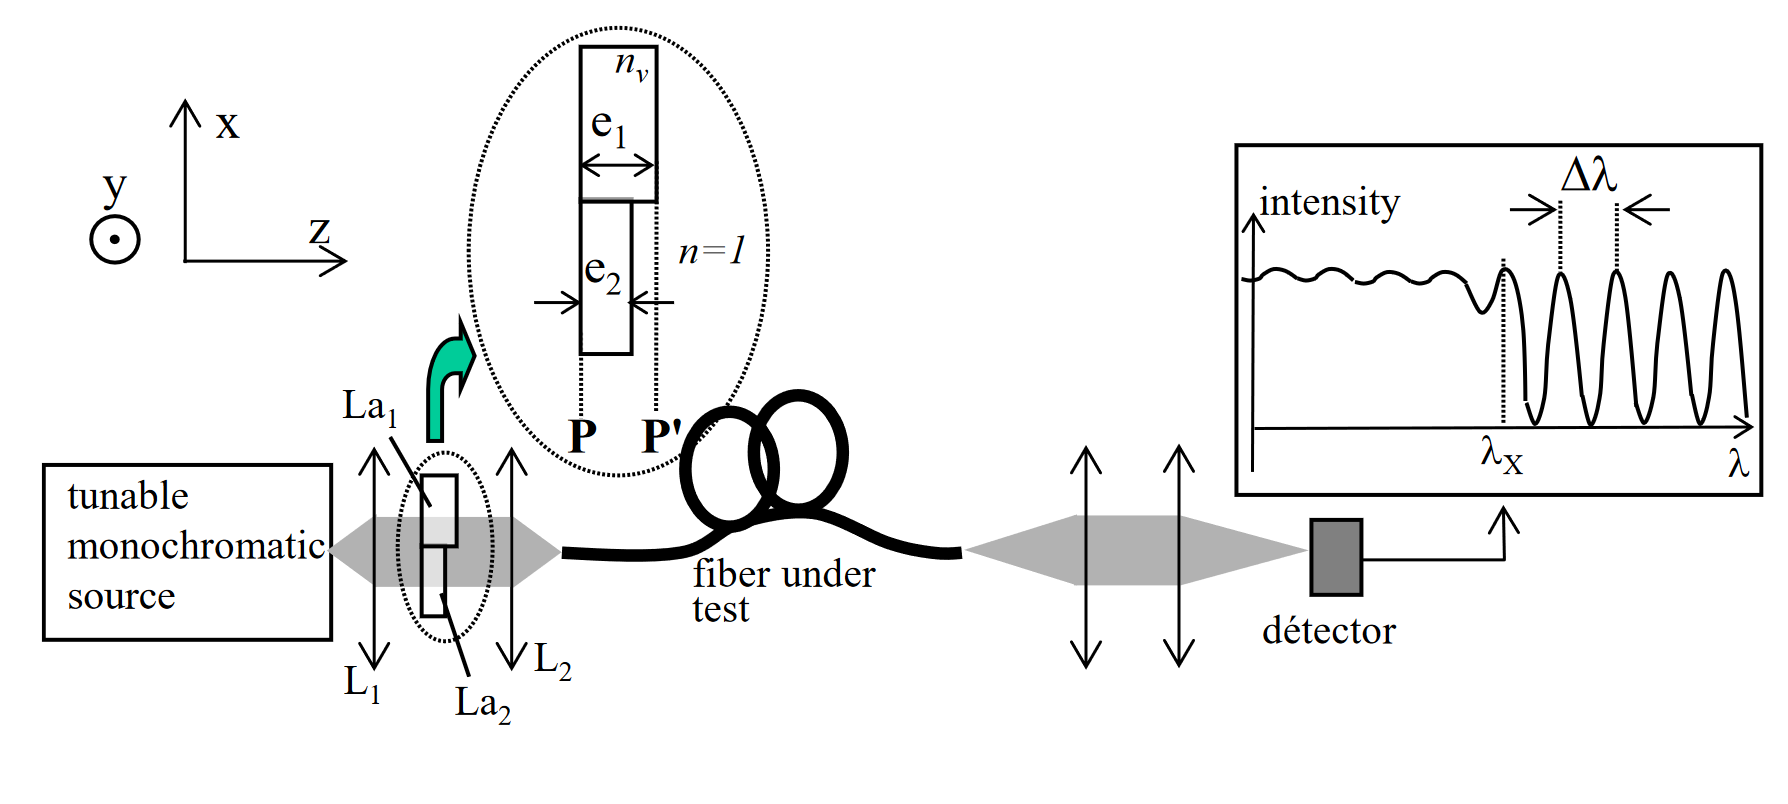
\includegraphics[width=16cm]{Images/Tutorial-Two-setup.png}
	\caption{Tutorial Two Experimental Set-up}  %% Caption for your figure
	\label{fig:tutorial_two_setup}
\end{figure}


\textit{The source is a monochromatic source, linearly polarized in the x direction. The emitted wavelength can be selected in the range 600nm-1700nm. The emitted power is supposed to remain constant whatever the selected wavelength. The output beam is collimated by a lens, $L_1$, in order to provide a plane wave, with a quasi-Gaussian spatial distribution of power. This plane wave is sent on an assembly of two glass plates set perpendicularly to the beam direction, and having a refractive index noted $n_v(\lambda)$ (index v stands for ``verre''; glass in French), as described in the figure above. Half of the beam crosses the plate $La_1$ of thickness $e_1$ and the second half crosses the plate $La_2$ of thickness $e_2$. The operating wavelength is $\lambda_T$.} \linebreak




%%%%% QUESTION FOUR %%%%%
\subsubsection{Question Four}

\paragraph{Part A \linebreak}
\textit{Verify that LP modes can be considered in the tested fibre. What is the meaning of ``LP''? What does it physically means?} \linebreak




\paragraph{Part B \linebreak}
\textit{Give the expression of the phase shift, $\delta\varphi_1$, experienced by the first half of the beam between the plane, $P$, and the plane, $P'$, as a function of the data of the problem.} \linebreak




\paragraph{Part C \linebreak}
\textit{Considering that the index of the air is 1, give the expression of the phase shift, $\delta\varphi_2$, experienced by the second half of the beam between the plane, $P$, and the plane, $P'$, as a function of the data of the problem.} \linebreak




\paragraph{Part D \linebreak}
\textit{Deduce that the phase difference, $\Delta\varphi$, between the two parts of the beam is given by Equation \ref{eqn:delta_varphi}:} \linebreak

\begin{equation}
	\Delta\varphi = \lvert \delta\varphi_1 - \delta\varphi_2 \rvert = \frac{2 \pi}{\lambda}(n_v(\lambda)-1)\Delta e \text{ where: } \Delta e = (e_1 - e_2)
	\label{eqn:delta_varphi}
\end{equation}




%%%%% QUESTION FIVE %%%%%
\subsubsection{Question Five}
\textit{Around the operating wavelength, we consider in first approximation that the refractive index of the plates is constant and is $n_v$.} \linebreak


\paragraph{Part A \linebreak}
\textit{Calculate the expression of the derivative of the phase difference, $\Delta\varphi$, with respect to the wavelength.} \linebreak




\paragraph{Part B \linebreak}
\textit{From this expression, deduce the literal expression of the free spectral range, $\Delta\lambda$, over which the phase difference, $\Delta\varphi$, varies by $2\pi$.} \linebreak




%%%%% QUESTION SIX %%%%%
\subsubsection{Question Six}
\textit{The beam exiting the assembly of plates is focused by means of the lens $L_2$ on the core of the fibre. It is perfectly centred on this core and there is no angular tilt. We still work at $\lambda_{T1}$ = 1100nm. We know that, at $\lambda_{T1}$, the fibre is able to guide only two LP modes.} \linebreak


\paragraph{Part A \linebreak}
\textit{What are these modes? Plot a schematic representation of the spatial distribution of the intensity of light in each of these modes.} \linebreak




\paragraph{Part B \linebreak}
\textit{Plot, for each mode, few lines of the electric field in the plane, at any moment.} \linebreak




%%%%% QUESTION SEVEN %%%%%
\subsubsection{Question Seven}
\textit{we assume that, at $\lambda_{T1}$, $\Delta\varphi = 2 m \pi$ (m is an integer). What mode will be mainly excited in the fibre? What will be the part of the energy which will be coupled in the $LP_{11}$ mode? Justify your answers.} \linebreak




%%%%% QUESTION EIGHT %%%%%
\subsubsection{Question Eight}
\textit{The source now emits light at the wavelength $\lambda_{T2}$ = 1102.4nm. What is the value of $\Delta\varphi$? Now, what mode will be mainly excited in the fibre? What will be the part of the energy which will be coupled in the $LP_{01}$ mode? Justify your answers.} \linebreak




%%%%% QUESTION NINE %%%%%
\subsubsection{Question Nine}
\textit{When the wavelength emitted by the source is increased little by little, we first note only little fluctuations of the detected power, with a period equal to $\Delta\lambda$. Then, beyond a wavelength, $\lambda_x$, the fluctuations of the detected power become very large, and this detected power even reaches zero for certain wavelengths spaced by de $\Delta\lambda$ (see the inset in the Figure \ref{fig:tutorial_two_setup} above).} \linebreak


\paragraph{Part A \linebreak}
\textit{With the help of the answers to questions 7 and 8, explain the origin of these large fluctuations.} \linebreak




\paragraph{Part B \linebreak}
\textit{To what parameter corresponds $\lambda_x$? Finally, what kind of characterization is achieved by means of the set-up described on Figure \ref{fig:tutorial_two_setup}?} \linebreak




%%%%% QUESTION TEN %%%%%
\subsubsection{Question Ten}
\textit{The cut-off wavelength of the second mode is $\lambda_c$ = 1240nm.} \linebreak


\paragraph{Part A \linebreak}
\textit{What is the radius of the core of the fibre?} \linebreak




\paragraph{Part B \linebreak}
\textit{We now work at $\lambda_{T2}$ = 633 nm. What are the LP modes able to propagate in the fibre? Justify your answer.} \linebreak




\paragraph{Part C \linebreak}
\textit{Determine the effective index of the lowest order mode and of the highest order mode able to propagate and calculate their respective phase velocities.} \linebreak




%%%%% TUTORIAL THREE %%%%%
\subsection{Tutorial Three - Part A: Birefringence and Polarization Mode Dispersion}
\textit{One can show that the normalized phase birefringence $B_{\varphi}$ of an optical fibre having an optical core and working in the single mode regime depends on the wavelength following the relation:  $B_{\varphi} = \sigma \cdot \lambda^2$, where $\sigma$ is a constant.} \linebreak




%%%%% QUESTION ONE %%%%%
\subsubsection{Question One}
\textit{What is the relation existing between $B_{\varphi}$ and the effective indices $n_{ex}$ and $n_{ey}$ of the two polarization modes ($HE_{11x}$  and  $HE_{11x}$, x and y being the directions of the two neutral axes (or eigen-axes) of the fibre)?} \linebreak




%%%%% QUESTION TWO %%%%%
\subsubsection{Question Two}
\textit{Show that the beat length $L_B$ between these two modes can be written: $L_B = \frac{\lambda}{B_{\varphi}}$} \linebreak




%%%%% QUESTION THREE %%%%%
\subsubsection{Question Three}
\textit{We work at $\lambda$ = 1.55$\mu m$. The effective index of the mode polarized along one of the eigen-axis is 1.4455 and $L_B$ = 3mm. Calculate the constant $\sigma$ (USI) and deduce the possible values of the effective index of the mode polarized in the orthogonal direction, rounded to the nearest $10^{-5}$} \linebreak




%%%%% QUESTION FOUR %%%%%
\subsubsection{Question Four}
\textit{Show that, for this fibre, the group birefringence $B_G$ can be expressed very simply versus $B_{\varphi}$. Give its value at $\lambda = 1.55 \mu m$} \linebreak




%%%%% QUESTION FIVE %%%%%
\subsubsection{Question Five}
\textit{The group index of the mode polarized in the direction \circled{1} is $N_{g}\circled{1} = 1.4722$ ( \circled{1} = x or y). Calculate $N_{g}\circled{2}$ ( \circled{2} = y or x, respectively) to the nearest $10^{-5}$, $N_{g}\circled{2}$ being the group index of the mode polarized in the orthogonal direction, knowing that $N_{g}\circled{2} \geq N_{g}\circled{1}$} \linebreak




%%%%% QUESTION SIX %%%%%
\subsubsection{Question Six}
\textit{A short light pulse with a triangular $P(t)$ shape, $P$ being the power, is emitted by a laser. The full width at half maximum (FWHM) of this pulse is 1ps. The pulse is launched into the studied fibre after crossing a polariser oriented at $45^{\circ}$ to the neutral axes of the fibre. What proportion of the energy propagating in the fibre is carried by the $HE_{11x}$ mode and by the $HE_{11y}$ mode? We neglect the effects of the chromatic dispersion and we consider that the fibre behaves as a polarisation maintaining fibre; represent the temporal shape of the signal detected at the output, after a 10m long propagation in the fibre.} \linebreak




%%%%% TUTORIAL THREE %%%%%
\subsection{Tutorial Three - Part B: Chromatic Dispersion}
\textit{A silica step index fibre is used for a high bit rate transmission @ $\lambda_T$ = 1.55$\mu m$. This fibre is single mode at the working wavelength $\lambda_T$. The effective index of the fundamental mode can take the following form around $\lambda_T$: $n_e(\lambda) = A_2 \lambda^2 + A_1 \lambda + A_0$, where $A_2$, $A_1$, and $A_0$ are constant values.} \linebreak




%%%%% QUESTION ONE %%%%%
\subsubsection{Question One}
\textit{A short pulse centred at $\lambda_T$ takes exactly 0.491317 ms for travelling over a distance of 100km in the fibre.} \linebreak




\paragraph{Part A \linebreak}
\textit{What is the value of the group velocity in the fibre @ $\lambda_T$?} \linebreak




\paragraph{Part B \linebreak}
\textit{Calculate the group index at $\lambda_T$, with a precision of $10^{-5}$.} \linebreak




%%%%% QUESTION TWO %%%%%
\subsubsection{Question Two}
\paragraph{Part A \linebreak}
\textit{Show that the expression of the group index as a function of the effective index, $n_e$, and the wavelength is $n_g = n_e - \lambda \frac{d n_e}{d \lambda}$} \linebreak




\paragraph{Part B \linebreak}
\textit{Express the group index versus $A_2$, $A_1$, $A_0$, and $\lambda$.} \linebreak




\paragraph{Part C \linebreak}
\textit{The parameter $A_0$ is equal to 1.47. Show that $A_2 = -16.45 \times 10^{-4} \mu m^{-2}$} \linebreak




%%%%% QUESTION THREE %%%%%
\subsubsection{Question Three}
\textit{The chromatic dispersion D of the fundamental mode can be expressed under the form $D_c = \frac{1}{c} \frac{d n_g}{d \lambda}$} \linebreak




\paragraph{Part A \linebreak}
\textit{Show that $D_c = - \frac{\lambda}{c} \frac{d^2 n_g}{d \lambda^2}$} \linebreak




\paragraph{Part B \linebreak}
\textit{Calculate the chromatic dispersion of the fibre at $\lambda_T$, expressed in the usual unit system: ps/(km.nm)} \linebreak




%%%%% QUESTION FOUR %%%%%
\subsubsection{Question Four}
\textit{At $\lambda_T$, the dispersion of silica is $D_m$ = 22 ps/(km.nm)} \linebreak




\paragraph{Part A \linebreak}
\textit{Why is the chromatic dispersion of the fibre different from the dispersion of silica ($D_c \neq D_m$)?} \linebreak




\paragraph{Part B \linebreak}
\textit{With what means can the manufacturers adjust the chromatic dispersion of the guided mode, at a given wavelength?} \linebreak




%%%%% QUESTION FIVE %%%%%
\subsubsection{Question Five}
\textit{Calculate the propagation length L at the end of which a pulse having an initial duration $\Delta$t = 150ps and a spectral width equal to $\sigma_{\lambda}$ = 0.3nm will have its duration increased by 50\%.} \linebreak




\newpage




%%%%% TUTORIAL FOUR %%%%%
\subsection{Tutorial Four - Chromatic Dispersion in a Step Index Fibre}
\textit{Let us remind that the group index at the wavelength } \linebreak




\newpage
\setstretch{1}  % Reduce bibliography line spacing
\bibliographystyle{IEEETran}
\bibliography{references.bib}
\end{document}
